% thesis_main.tex
%
% You don't need to change this file unless you use a different number
% of chapters than the template. See the EDIT HERE line below.
%
% 
%\documentclass[12pt,dblspace]{report}
\documentclass[12pt]{report}

%\usepackage{url}
\usepackage[hyphens]{url}
% \usepackage{subfigure}
\usepackage{multirow}
\usepackage[show]{chato-notes}
\usepackage{pdfpages}

\usepackage{natbib}
\usepackage[nottoc]{tocbibind}
\usepackage{datetime}
\usepackage{caption}
\usepackage{subcaption}

%\usepackage{geometry} 
\usepackage[margin=.8in]{geometry}
\usepackage{graphicx}
\usepackage{amssymb}
\usepackage[cmex10]{amsmath}
\usepackage{epstopdf}
\usepackage{setspace}
\usepackage{listings}
\usepackage{amsthm}
\usepackage{url}
\usepackage{float}
\usepackage{hyperref}
\usepackage{tikz}
\usetikzlibrary{fit,positioning}

% macros of Wei-Lwun
% =============================================================================
% New commands
% -----------------------------------------------------------------------------


\newcommand{\eg}{\emph{e.g.}\@\xspace}
\newcommand{\ie}{\emph{i.e.}\@\xspace}

\makeatletter
\newcommand{\etc}{%
    \@ifnextchar{.}%
        {\emph{etc}}%
        {\emph{etc.}\@\xspace}%
}
\newcommand{\etal}{%
    \@ifnextchar{.}%
        {\emph{et al}}%
        {\emph{et al.}\@\xspace}%
}
\makeatother


\newcommand{\vect}[1]{\boldsymbol{#1}}
\newcommand{\argmax}[1]{\underset{#1}{arg\,max}\,\,}
\newcommand{\argmin}[1]{\underset{#1}{arg\,min}\,\,}
\newcommand{\expect}[1]{\langle #1 \rangle}
\newcommand{\normone}[1]{\| #1 \|_1}
\newcommand{\meanvar}[2]{#1\,{\scriptsize (#2)}}
\newcommand{\bigspace}[0]{\;\;\;\;\;\;\;\;\;\;\;\;\;\;\;\;\;\;\;\;\;\;\;\;\;\;\;\;\;\;\;\;\;\;\;\;\,}
\newcommand{\naive}{na\"ive }
\newcommand{\refeq}[1]{Eq.~(\ref{#1})}
\newcommand{\reffig}[1]{Figure \ref{#1}}
\newcommand{\what}[1]{\widehat{#1}}


% Mathmatics (from Kevin Murphy)
\newcommand{\be}{\begin{equation}}
\newcommand{\ee}{\end{equation}}

\newcommand{\myvec}[1]{\mbox{$\mathbf{#1}$}}
\newcommand{\myvecsym}[1]{\mbox{$\boldsymbol{#1}$}}

\newcommand{\vzero}{\mbox{$\myvecsym{0}$}}
\newcommand{\vone}{\mbox{$\myvecsym{1}$}}

\newcommand{\valpha}{\mbox{$\myvecsym{\alpha}$}}
\newcommand{\vbeta}{\mbox{$\myvecsym{\beta}$}}
\newcommand{\vdelta}{\mbox{$\myvecsym{\delta}$}}
\newcommand{\vepsilon}{\mbox{$\myvecsym{\epsilon}$}}
\newcommand{\veta}{\mbox{$\myvecsym{\eta}$}}
\newcommand{\vgamma}{\mbox{$\myvecsym{\gamma}$}}
\newcommand{\vmu}{\mbox{$\myvecsym{\mu}$}}
\newcommand{\vlambda}{\mbox{$\myvecsym{\lambda}$}}
\newcommand{\vLambda}{\mbox{$\myvecsym{\Lambda}$}}
\newcommand{\vphi}{\mbox{$\myvecsym{\phi}$}}
\newcommand{\vPhi}{\mbox{$\myvecsym{\Phi}$}}
\newcommand{\vpi}{\mbox{$\myvecsym{\pi}$}}
\newcommand{\vPsi}{\mbox{$\myvecsym{\Psi}$}}
\newcommand{\vtheta}{\mbox{$\myvecsym{\theta}$}}
\newcommand{\vTheta}{\mbox{$\myvecsym{\Theta}$}}
\newcommand{\vsigma}{\mbox{$\myvecsym{\sigma}$}}
\newcommand{\vSigma}{\mbox{$\myvecsym{\Sigma}$}}
\newcommand{\vtau}{\mbox{$\myvecsym{\tau}$}}
\newcommand{\vxi}{\mbox{$\myvecsym{\xi}$}}

\newcommand{\va}{\mbox{$\myvec{a}$}}
\newcommand{\vb}{\mbox{$\myvec{b}$}}
\newcommand{\vc}{\mbox{$\myvec{c}$}}
\newcommand{\vd}{\mbox{$\myvec{d}$}}
\newcommand{\ve}{\mbox{$\myvec{e}$}}
\newcommand{\vf}{\mbox{$\myvec{f}$}}
\newcommand{\vg}{\mbox{$\myvec{g}$}}
\newcommand{\vh}{\mbox{$\myvec{h}$}}
\newcommand{\vj}{\mbox{$\myvec{j}$}}
\newcommand{\vk}{\mbox{$\myvec{k}$}}
\newcommand{\vm}{\mbox{$\myvec{m}$}}
\newcommand{\vn}{\mbox{$\myvec{n}$}}
\newcommand{\vp}{\mbox{$\myvec{p}$}}
\newcommand{\vq}{\mbox{$\myvec{q}$}}
\newcommand{\vr}{\mbox{$\myvec{r}$}}
\newcommand{\vs}{\mbox{$\myvec{s}$}}
\newcommand{\vt}{\mbox{$\myvec{t}$}}
\newcommand{\vu}{\mbox{$\myvec{u}$}}
\newcommand{\vv}{\mbox{$\myvec{v}$}}
\newcommand{\vw}{\mbox{$\myvec{w}$}}
\newcommand{\vx}{\mbox{$\myvec{x}$}}
\newcommand{\vxt}{\mbox{$\myvec{\tilde{x}}$}}
\newcommand{\vy}{\mbox{$\myvec{y}$}}
\newcommand{\vyt}{\mbox{$\myvec{\tilde{y}}$}}
\newcommand{\vz}{\mbox{$\myvec{z}$}}

\newcommand{\vA}{\mbox{$\myvec{A}$}}
\newcommand{\vB}{\mbox{$\myvec{B}$}}
\newcommand{\vC}{\mbox{$\myvec{C}$}}
\newcommand{\vD}{\mbox{$\myvec{D}$}}
\newcommand{\vE}{\mbox{$\myvec{E}$}}
\newcommand{\vF}{\mbox{$\myvec{F}$}}
\newcommand{\vG}{\mbox{$\myvec{G}$}}
\newcommand{\vH}{\mbox{$\myvec{H}$}}
\newcommand{\vI}{\mbox{$\myvec{I}$}}
\newcommand{\vJ}{\mbox{$\myvec{J}$}}
\newcommand{\vK}{\mbox{$\myvec{K}$}}
\newcommand{\vL}{\mbox{$\myvec{L}$}}
\newcommand{\vM}{\mbox{$\myvec{M}$}}
\newcommand{\vN}{\mbox{$\myvec{N}$}}
\newcommand{\vO}{\mbox{$\myvec{O}$}}
\newcommand{\vP}{\mbox{$\myvec{P}$}}
\newcommand{\vQ}{\mbox{$\myvec{Q}$}}
\newcommand{\vR}{\mbox{$\myvec{R}$}}
\newcommand{\vS}{\mbox{$\myvec{S}$}}
\newcommand{\vT}{\mbox{$\myvec{T}$}}
\newcommand{\vU}{\mbox{$\myvec{U}$}}
\newcommand{\vV}{\mbox{$\myvec{V}$}}
\newcommand{\vW}{\mbox{$\myvec{W}$}}
\newcommand{\vX}{\mbox{$\myvec{X}$}}
\newcommand{\vY}{\mbox{$\myvec{Y}$}}
\newcommand{\vZ}{\mbox{$\myvec{Z}$}}

% bar
\newcommand{\vgbar}{\mbox{$\overline{\vg}$}}
\newcommand{\vxbar}{\mbox{$\overline{\vx}$}}
\newcommand{\vybar}{\mbox{$\overline{\vy}$}}
\newcommand{\vzbar}{\mbox{$\overline{\vz}$}}
\newcommand{\vpbar}{\mbox{$\overline{\vp}$}}
\newcommand{\vbbar}{\mbox{$\overline{\vb}$}}

% displacement
\newcommand{\dvc}{\mbox{$\delta\vc$}}

% partial derivative
\newcommand{\pvr}{\mbox{$\partial\vr$}}
\newcommand{\pvc}{\mbox{$\partial\vc$}}

% probability distributions
\newcommand{\betadist}{\mbox{Beta}}
\newcommand{\bernoulli}{\mbox{Ber}}
\newcommand{\Ber}{\mbox{Ber}}
\newcommand{\Binom}{\mbox{Bin}}
\newcommand{\binomdist}{\mbox{Bin}}
\newcommand{\Dir}{\mbox{Dir}}
\newcommand{\discrete}{\mbox{discrete}}
\newcommand{\Discrete}{\mbox{Discrete}}
\newcommand{\expdist}{\mbox{Exp}}
\newcommand{\gammadist}{\mbox{Ga}}
\newcommand{\Ga}{\mbox{Ga}}
\newcommand{\gauss}{\mbox{${\cal N}$}}
\newcommand{\IG}{\mbox{IG}}
\newcommand{\Mu}{\mbox{Mu}}
\newcommand{\Multi}{\mbox{Mu}}
\newcommand{\NIX}{\mbox{$NI\chi^2$}}
\newcommand{\NIG}{\mbox{NIG}}
\newcommand{\NGdist}{\mbox{NG}}
\newcommand{\prob}{\mbox{$p$}}
\newcommand{\Poi}{\mbox{Poi}}
\newcommand{\Student}{\mbox{${\cal T}$}}
\newcommand{\student}{\mbox{${\cal T}$}}
\newcommand{\Wishart}{\mbox{Wi}}
\newcommand{\Wi}{\mbox{Wi}}

% =============================================================================

% =============================================================================
% Renew commands
% -----------------------------------------------------------------------------
\renewcommand{\min}[1]{\underset{#1}{min}\,\,}
\renewcommand{\max}[1]{\underset{#1}{max}\,\,}
% =============================================================================


\floatstyle{plain} 
%\floatstyle{boxed}
\restylefloat{figure}

\DeclareGraphicsRule{.tif}{png}{.png}{`convert #1 `dirname #1`/`basename #1 .tif`.png}
\hsize=5in
\vsize=7.5in
%\hoffset=.05in
\voffset=.0in
%\hoffset=.25in
%\voffset=.25in
\renewcommand{\baselinestretch}{1}
%\renewcommand{\baselinestretch}{2}

%
% To get page numbering exactly right (not really needed),
% Uncomment next line after editing toc and lof files appropriately.
%\nofiles
%





\newcommand{\mychapter}[1]{\newpage \vspace*{0.00mm} \refstepcounter{chapter} 
	
	{\LARGE \bf  \noindent \thechapter \hspace*{0.5em}   
		#1\baselineskip=1.0\normalbaselineskip\par}
	
			\vspace*{3ex} \par 
\addcontentsline{toc}{chapter}{\protect \numberline{\thechapter}{#1}}   }


%\newcommand{\mychapter}[1]{\newpage \vspace*{0.01mm} \refstepcounter{chapter} 
%	\begin{center}
%	{\huge \bf Chapter \space  \thechapter \vspace*{1em}  \par 
%		#1\baselineskip=1.0\normalbaselineskip\par}
%		 \end{center} 
%			\vspace*{3ex} \par 
%\addcontentsline{toc}{chapter}{\protect \numberline{\thechapter}{#1}}   }


%\newcommand{\myappendix}[1]{\newpage \vspace*{0.01mm} \refstepcounter{chapter}
%        \begin{center}
%        {\LARGE \bf Appendix \space  \thechapter \vspace*{1em}  \par
%                #1\baselineskip=1.0\normalbaselineskip\par}
%                 \end{center}
%                        \vspace*{3ex} \par
%\addcontentsline{toc}{chapter}{Appendix \protect \numberline{\thechapter} - {#1} } }

\pagenumbering{arabic}
\setcounter{page}{1}
\pagestyle{myheadings}
\begin{document}
\renewcommand{\baselinestretch}{1.3}
%\renewcommand{\baselinestretch}{1.3}

% \input epsf

\setlength{\headsep}{0.15in}
%\setlength{\headsep}{1.15in}
\setlength{\topmargin}{-.5in}
\pagenumbering{roman}
\pagestyle{empty}



\title{
\textbf{Question Answering Using Structured and Unstructured Data} \\
%\textbf{Improving Information Access with Community Question Answering} \\
\normalfont Doctoral thesis proposal}
\author{\textbf{Denis Savenkov}\\
      Dept. of Math \& Computer Science\\
      Emory University\\
      denis.savenkov@emory.edu
}


\newdateformat{mydate}{\monthname[\THEMONTH], \THEYEAR}

\mydate

\maketitle


\begin{abstract}



Modern search engines have made a dramatic progress in answering many users questions, especially about facts, such as those that might be retrieved or directly inferred from a knowledge base.
However, many other questions that real users ask, \eg more complex factual, opinion or advice questions, are still largely beyond the competence of computer systems.
For such information needs users still have to dig deeper into the ``10 blue links'' and extract relevant pieces of information.
As conversational agents become more popular, question answering (QA) systems are increasingly expected to handle such complex questions and provide users with helpful and concise information.

Questions come in different flavors, some are asking about a certain fact and can be answered with a short phrase, such as entity name, date or number.
Such questions are typically referred to as \textit{factoid}, while other types of questions are often called \textit{non-factoid}.
The goal of my thesis is to improve the performance of question answering systems for solving various users' information needs using different available data sources.
To achieve this goal I first focus on improving the question answering for factoid and non-factoid questions separately, and then study some aspects of the interaction between users and automated systems.
More specifically, the first part of the thesis studies how to combine available unstructured text and structured knowledge base (KB) data for factoid question answering, in the second I build a non-factoid QA system that improves different stages of a pipeline by utilizing available unstructured and semi-structured (\eg question-answer pairs) data, and the last part of the thesis address the problem of user experience for questions that a QA system could not answer.

Nowadays, there are a number of large open domain knowledge bases, that contain billions of facts about the world.
However, their incompleteness and problems mapping from natural language questions to the structured queries, limits their scope to only a small subset of user factoid information needs.
In my thesis I'm proposing a couple of new ways unstructured text data can be used to help knowledge base question answering.
First, I propose a novel relation extraction model, that compliment KB data with facts extracted from community question answer data.
And then, I describe a hybrid KB-Text QA system, that is based on semantic annotations of entity mentions in text documents.

Non-factoid question answering is somewhat harder as it deals with a more diverse set of question and answer types.
In my thesis I propose to improve performance of different stages of QA system pipeline by better utilization of the structure of a web page where a candidate answer is extracted from, and using deep learning techniques, inspired by recent successes in machine translation \cite{bahdanau2014neural}, text summarization \cite{rush-chopra-weston:2015:EMNLP}, automatic caption generation \cite{karpathy2015deep} and answer sentence scoring \cite{WangN15}.

Unfortunately, there will always be cases when a system is unable to answer user's questions, \eg it might be ambiguous.
In such cases a system can get back to the user with some kind of a suggestion or clarification.
The focus of the last part of the thesis is on how to engage in an interaction with a user to improve the overall QA experience.
I first describe strategic hints, which can help users to split complex information needs into smaller steps, which can be handled by the automated system.
Next, I describe the proposal of research for automatic generation of clarification questions, which a system can ask to resolve ambiguities in the original query.

In summary, the goal of the proposed research is to improve the performance of question answering over a variety of different questions a user might have, and to study some reply strategies in case a system fails to deliver a good response.
I believe, that results of the proposed work will be useful for the future research in improving automatic question answering.

%ThIS PART IS OLDER...

%Over the year of research most efforts were put on factoid questions, which can be answered with a short phrase, \eg an entity name, date, number, etc.
%Modern QA systems employ a variety of different unstructured (text-corpora), semi-structured (tables, Wikipedia infoboxes, question-answer pairs) and structured (databases, knowledge bases) data sources to generate candidate answers.
%Each of the data sources has its own advantages and limitations, in particular a text fragment encodes very limited amount of information about the entities involved in the statements, which complicates the reasoning about the answer correctness.
%For example, most factoid QA systems tries to substitute missing information with a prediction, \ie predict an expected lexical answer type (LAT) from the question and match it against the also predicted answer entity type.
%On the other side of the spectrum knowledge bases (KB) aggregate all available information about entities and support effective querying with a structured query language, such as SPARQL.
%The problem comes when we need to translate natural language information need to a structured query.
%Modern knowledge base question answering (KBQA) systems use question-answer pairs (QnA), question paraphrases and other resources to learn a lexicon to map from natural language phrases to knowledge base objects, which is still limited and works well for relatively popular simple questions.
%In addition knowledge bases are inherently incomplete and many entities, predicates and facts are simply missing.
%Therefore, it make sense to combine different data sources for question answering, and this approach was already shown to be successful by systems such as IBM Watson, but they treat different data sources mostly independently and use them to produce as a set of candidates, which are then ranked and the best answer is selected.
% However, for many questions it might be hard to find good candidates in the first place, and one would benefit from utilizing all available resources together at this stage.
%In my dissertation I propose to consider unstructured textual and structured knowledge base resources, connected via entity linking, together for joint reasoning on the candidate generation stage.
%Existing datasets for question answering are either relatively small (QALD tasks), focused on text (TREC QA) or on knowledge bases only (\eg WebQuestions).
%To evaluate the approach I'm going to build a new realistic dataset extracted from Yahoo! Answers question-answer pairs.

%Beyond factoid questions we have a plethora of different information needs, that require more than a simple fact to answer.
%Such questions are usually called non-factoid and more and more research effort is devoted to answering such questions.
%In 2015 Text REtrieval Conference (TREC) pioneered LiveQA shared task track, which targets automatic question answering of various types of questions user post on Yahoo! Answers Community Question Answering (CQA) website.
%Existing research has demonstrated the effectiveness of reusing answers to similar previously posted questions, but in many cases such questions are not available or challenging to find.
%Alternatively, existing systems rank passages extracted from regular web pages.
%However, ranking is complicated due to the lexical gap between question and answer text.
%Knowledge about what question does a paragraph of text answers would be very useful signal for ranking, which is supported by the results of the winning TREC LiveQA approach.
%In my thesis I propose to make a step further and automatically extract candidates text passages along with questions which they answers.
%This can be done by automatically detecting question-answer pairs from certain web pages (\eg forums, FAQ, \etc).
%In addition, we can build upon the recent success with automatic text generation by recurrent neural networks and train a model to predict a question for a given text fragment.

%In summary, this dissertation aims to improve the performance of automatic question answering systems for both factoid and non-factoid question answering.

\end{abstract}


\tableofcontents
%\listoffigures
%\listoftables




%%%%%%%%%%%%%%%%%%%%%%%%% EDIT HERE %%%%%%%%%%%%%%%%%%%%%%%%%%%%%%%%
% Change these lines to adjust for different numbers of chapters /
% appendices
%%%%%%%%%%%%%%%%%%%%%%%%%%%%%%%%%%%%%%%%%%%%%%%%%%%%%%%%%%%%%%%%%%%%
% chap1.tex
%
% First chapter file is different from others
%
\mychapter{Introduction}
\label{chap:intro}
\pagenumbering{arabic}
\setcounter{page}{1}
\pagestyle{myheadings}

%Uncomment to switch spacing.
%\baselineskip=5px

\newtheorem{definition}{Definition}
\newtheorem{proposition}{Proposition}


\section{Motivation}

% Information retrieval approaches for question answering over text collections were shown to be quite effective for factoid questions answering. However, the amount of information encoded in a text fragment is very limited, which makes inference and reasoning hard. 
% On the other hand, modern large scale knowledge bases encode vast amount of information about various entities and can answer all sorts of questions asked using structured query languages such as SPARQL. However, question answering over such linked data is complicated as we need to translate natural language questions into the structured form. In addition, knowledge base are incomplete and many entities, predicates and triples are simply missing.
% I propose to bridge the gap between the structured knowledge bases and unstructured text data for question answering by annotating documents with mentioned entities and extending the set of operations involved in question answering with operations traversing these links between knowledge base and text collections. For example, exploring the neighborhood of candidate answers from text documents in a KB brings additional information about the candidate, which can be matched against the parts of the question that is not stated in text. Alternatively, text fragments mentioning a given entity and some question terms can provide a link to another entity, that is currently missing in KB as well as additional signal for ranking.

% FROM WSDM DC

% Recently we witnessed some successes of QA systems, i.e. IBM Watson winning the Jeopardy! TV show, major companies adapting question answering technologies (Apple Siri, Google Now, Microsoft Cortana, etc). 
% However, these systems are still very limited and we have a lot to do to move beyond these 10 blue links in search results \cite{etzioni2011search} as for most of the questions users still have to dig into the retrieved documents or post questions to the community question answering (CQA) websites.

The ability to answer user questions with precise and concise information is a hard problem with a long history of research.
Various data sources are available for candidate answer generation, two major ones are unstructured text corpora, and structured knowledge bases (e.g. dpPedia \cite{auer2007dbpedia} and Freebase \cite{Bollacker:2008:FCC:1376616.1376746}).
A hybrid approach to question answering \cite{baudivs2015modeling,Ferrucci10:DeepQA} generates candidates from multiple sources, however each of them is typically processed separately and results are merged on the scoring and ranking stage when some information is already lost.
Efficient combination of different information sources has potential to improve both text and knowledge base question answering systems.
I propose to combine all the available sources together and do joint reasoning to generate better answer candidates and improve the overall question answering performance.

% Text-bases QA systems were shown to be quite effective on the TREC QA tasks as well as on other benchmark datasets \cite{dang2007overview}.
Question answering from text corpora typically starts by retrieving a set of potentially relevant documents using the question (or some transformation of the question \cite{AgichteinLG01}) as the query, and then extracting entities, phrases, sentences or paragraphs believed to be the answer to the question.
However, the information available in the retrieved pieces of text is very limited and often not enough to decide whether it can be the answer to the given question.
For example, below is one of the questions from TREC QA 2007 dataset:\\
\textit{``What republican senators supported the nomination of Harriet Miers to the Supreme Court?''}\\
A candidate answer sentence \textit{``Minority Leader Harry Reid had already offered his open support for Miers.''} mentions a senator ``Harry Reid'' and clearly says about his support of the nomination.
However, ``Harry Reid'' is not a correct answer to the question because he is a member of the Democratic party.
This information is not available in the answer candidate sentence, but it is present as one of the properties in Freebase: [Harry Reid, political\_party, Democratic party]\footnote{Actually, in Freebase the entities are connected by a path of length 2 through a mediator node. The predicates on the path are: /government/politician/party and /government/political\_party\_tenure/party}.
Therefore, by looking into the knowledge available about the mentioned entities a QA system can make a better judgment about the candidate answer.

Question answering over linked data (knowledge bases) converts a natural language question into a structured query, such as SPARQL.
The main challenge for such systems is to map words and phrases from the question to the corresponding entities and predicates from a KB.
Usually, such lexicon is built during training using ground truth question-query pairs \cite{CaiY13} or question-answer pairs \cite{BerantCFL13:sempre}.
Improvements were made by extending the lexicon using Wikipedia and patterns expressing certain predicates obtained via distant supervision \cite{bastmore:cikm:2015:aquu,BordesCW14:emnlp,ReddyLS14,yih:ACL:2015:STAGG,YaoD14}.
But still, the amount of available labeled or weakly labeled training data is much smaller than the amount of unstructured data.
This unstructured data will complement the learned lexicon, e.g. even if a question about a certain predicate wasn't seen during training, a set of text paragraphs mentioning both of the related entities can provide a QA system with enough evidence to make the correct decision.

Table \ref{table:data_procons} lists pros and cons of structured and unstructured data sources for factoid and non-factoid question answering.

\begin{table*}
\centering
\caption{Pros and cons of structured and unstructured data sources for factoid and non-factoid question answering}
\begin{tabular}{| l | p{6cm} | p{6cm} |}
\hline
 & unstructured data & structured data \\
\hline
factoid questions & \multicolumn{1}{|c|}{Text} & \multicolumn{1}{|c|}{Knowledge Bases} \\
 & + easy to match against question text & + aggregate all the information about entities\\
 & + cover a variety of different information types & allow complex queries over this data using special languages (e.g. SPARQL) \\
 & - each text phrase encodes a limited amount of information about mentioned entities & - hard to translate natural language questions into special query languages \\
&  & - KBs are incomplete (missing entities, facts and properties) \\
\hline
non-factoid questions & \multicolumn{1}{|c|}{Text} & \multicolumn{1}{|c|}{Question-Answer pairs} \\
 & + contain relevant information to a big chunk of user needs & + easy to find a relevant answer by matching the corresponding questions \\
 & - hard to extract semantic meaning of a paragraph to match against the question (lexical gap) & - cover a smaller subset of user information needs \\
\hline
\end{tabular}
\label{table:data_procons}
\end{table*}


The main focus of research in automatic question answering was on \textbf{factoid questions}, which inquire about a certain fact and can be answered with a short phrase, such as an entity name, date or number.
Such questions cover, although big and an important, but only a fraction of user information needs.
Questions that don't fall into this category are usually referred to as \textbf{non-factoid}.


\section{Research Questions}


\section{Research Plan}

\subsection{Step 1 (Chapter 3)}
\label{sec:plan1}

\subsection{Step 2 (Chapter 4)}
\label{sec:plan2}

\subsection{Step 3 (Chapter 5)}
\label{sec:plan3}

\subsection{Research Timeline}

% \noindent A tentative timeline for the work that needs to be done is shown below:

%\begin{itemize}
%\item Completing the work proposed in Section \ref{sec:plan2} (10/2013 - 11/2013): For detecting implicit question intent in web search, build a better evaluation set, develop more features for the classifier and compare with more baselines.
%\item Completing the work proposed in Section \ref{sec:plan3} (12/2013 - 04/2014): For improving question search for queries with question intent, develop models that build better query model and learn better word-to-word translation relationships based on the query-question click data and question category information.
%\item \textbf{If time permits}, extending the work proposed in Section \ref{sec:plan3} (03/2014 - 04/2014): Extend the methods developed above for question search to achieve better query expansion and results ranking for general web search.
%\item Thesis writing (05/2014 - 08/2014) 
%\item Thesis defense (08/2014)
%\end{itemize}


\section{Contributions and Implications}

The key contributions of the proposed research are:
1. New hybrid KB-text question answering algorithm, that is based on graph search, which includes both KB links as well as text search edges to follow.
2. New labelled dataset for question answering (???)
3. New features for ranking answer candidates ???

% chap2.tex
%

\mychapter{Related Work}
\label{chap:related}

Some useful materials for the related work section:
\begin{itemize}
\item https://web.stanford.edu/$\sim$jurafsky/slp3/28.pdf
\item PhD thesis ``FEATURE-DRIVEN QUESTION ANSWERING WITH NATURAL LANGUAGE ALIGNMENT''
\end{itemize}


% The field of question answering has a long history of research and dates back to 60s, when first systems attempted to provide a natural language interface to databases \cite{Simmons:1965:AEQ:363707.363732}.
% In 70s and 80s the development of restricted domain knowledge bases set a task for question answering frameworks to assist users in solving their problem, which lead to the development of interactive question answering systems, e.g. \cite{shortliffe1976mycin}, \cite{woods1977lunar}.

% The modern era of question answering research started with the rise of the Internet and exponential growth of information available in the World Wide Web.
% Since 1999 the annual Text Retrieval Conference (TREC)\footnote{http://trec.nist.gov} organized a number of open domain question answering shared tasks, e.g. see \cite{dang2007overview} for a review.
% In 2015 TREC piloted a LiveQA track\footnote{http://trec-liveqa.org/}, in which the participant systems had to answer various questions coming from real users of Yahoo! Answers\footnote{http://answers.yahoo.com/} in real time.

The field of question answering has a long history of research and dates back to 60s (see \cite{Kolomiyets:2011:SQA:2046840.2047162} for a survey of different approaches).
The modern era of question answering research started with the rise of the Internet and exponential growth of information available in the World Wide Web.
Since 1999 the annual TREC organized a number of open domain question answering shared tasks \cite{dang2007overview}.
Approaches proposed over the years can be largely classified by the type of the information used to find the answers into knowledge base and text-based systems.

\section{Text-based QA}

A traditional approach to factoid question answering over document collections popularized by the TREC QA track is to retrieve a set of potentially relevant documents, extract and rank mentioned entities as candidate answers.
One of the main challenges of such an approach is limited amount of information present in the extracted pieces of text.
Systems test answer for incorrectness by matching the expected answer type with the type of candidate entity often predicted by an named entity tagger.
These systems rely heavily on special complicated ontologies that encode the relationships between different question and answer types, e.g. \cite{hovy2000question,LiRoth02, prager2006question}.
Alternatively, the AskMSR system \cite{brill_askmsr} (recently reviewed in \cite{tsai2015web}) used the redundancy of large text collections such as the web to extract n-grams that occur frequently in a retrieved set of documents.
Their counting-based approach performed unexpectedly well on TREC 2001 and sparkled an interest in exploring the web for question answering purposes \cite{LinK03}.
However, in many cases the information from the extracted text fragments is not enough to make a judgment on an answer candidate.
To solve this problem researchers experimented with using external resources, both unstructured (e.g. Wikipedia articles  \cite{ahn2005using, buscaldi2006mining}) and structured (e.g. Wordnet \cite{pasca2001informative}), and demonstrated improved question answering performance.
Recently \cite{Sun:2015:ODQ:2736277.2741651} proposed to link entities from candidate answers to Freebase and use its type system and textual entity description for candidate scoring.
However, most of the information in a KB is stored as relations between entities, therefore there is a big potential in using all available KB data to improve question answering.

\section{Knowledge base QA}

Recent development of large scale knowledge bases (e.g. dbPedia \cite{auer2007dbpedia}) and Freebase \cite{Bollacker:2008:FCC:1376616.1376746}) motivated research in open domain question answering over linked data.
Developed models can be compared on the annual QALD shared task \footnote{http://greententacle.techfak.uni-bielefeld.de/$\sim$cunger/qald/} and on a number of available benchmark datasets, e.g. WebQuestions \cite{BerantCFL13:sempre}.
The main challenge of such systems is to map natural language questions into the structured query representation.
Such a lexicon can be learned from a labeled training set \cite{BerantCFL13:sempre},  ClueWeb collection aligned to Freebase \cite{ReddyLS14,YaoD14}, question paraphrases clusters from WikiAnswers \cite{BerantL14:parasempre}, Freebase triples rephrased as questions \cite{BordesCW14:emnlp}, and can be based on the embeddings of questions and knowledge base entities and predicates \cite{BordesCW14:emnlp,yih:ACL:2015:STAGG}.
However, most of the models are still biased towards the types of questions present in the training set and would benefit from more training data.
In this work I propose to extend the training set with question-answer pairs available on CQA websites, which were shown to be useful for relation extraction \cite{SavenkovLDA15}.
In addition, I propose to use unlabeled text resources for candidate query ranking, which can help to generalize to unseen types of questions and questions about predicates never mentioned in the training set.

\section{Hybrid techniques}

Hybrid question answering systems combine multiple available information sources, in particular text document and knowledge bases.
Examples of such systems include IBM Watson \cite{Ferrucci10:DeepQA}, OpenQA \cite{Fader:2014:OQA:2623330.2623677}, YodaQA \cite{baudivs2015modeling}.
The main difference between such systems and the proposed research is that hybrid systems typically use separate pipelines to extract candidates from different sources and only merge the candidate set while ranking.
I propose to extend the representation of each of the data sources for better candidate generation from the beginning.


\clearpage
% chap3.tex
%

\mychapter{Structured and Unstructured Data for Factoid Question Answering}
\label{chapter:factoid}

\noindent

There are multiple ways to marry unstructured and structured data for joint question answering: convert structured data to unstructured format or vice versa, convert all data to certain intermediate representation or to leave them as is and link the data sources.
In my thesis I focus on two approaches: relation extraction for knowledge base completion, and semantic annotation of text for hybrid question answering.

% =-=-=-=-=-=-=-=-=-=-=-=-=-=-=-=-=-=-=-=-=-=-=-=-=-=-=-=-=-=-=-=-=-=-=-=-=-

\section{Relation Extraction for Knowledge Base Completion}
\label{sec:relation_extraction}

The information on the web is stored in multiple different forms, such as natural language statements, tables and infoboxes, images \etc.
In this work I focus on yet another source of information: question-answer pairs.
Community question answering archives contain hundreds of millions of question and corresponding answers.
Information expressed in these pairs might be hard to extract or not exist at all in other formats.

\subsection{Relation extraction from Question-Answer pairs}
\label{subsec:cqa_relextract}

CQA websites, such as Yahoo! Answers\footnote{http://answers.yahoo.com/}, Answers.com\footnote{http://www.answers.com}, Quora\footnote{http://quora.com} \etc, has gained a lot of popularity in the recent years, and their archives store hundreds of millions of user questions along with answers provided by the community.
Many users' information needs are not unique and arise again and again, which makes it possible to reuse the information to answers new questions \cite{Shtok:2012:LPA:2187836.2187939}.
This idea makes CQA data attractive for knowledge base population.
Although some of the facts mentioned in QnA pairs can also be found in some other text documents, another part might be unique (\eg in Clueweb\footnote{http://www.lemurproject.org/clueweb12/} about 10\% of entity pairs with existing Freebase relations mentioned in Yahoo! Answers documents cannot be found in other documents \cite{savenkov2015relation}).
Existing relation extraction techniques face some challenges when applied to CQA data, \ie they typically consider sentences independently and ignore the discourse of a QnA pair text.
However, frequently, it is impossible to understand the answer without knowing the question.
For example, sometimes users simply give the answer to the question without stating it in a narrative sentence (\eg ``\emph{What does "xoxo" stand for? Hugs and kisses.}``), or the provided answer might contain ellipsis, \ie some important information is omitted (\eg ``\emph{What's the capital city of Bolivia? Sucre is the legal capital, though the government sits in La Paz}``).

In this thesis we propose a novel model for relation extraction from CQA data, that uses discourse of a QnA pair to extract facts between entities mentioned in question and entities mentioned in answer sentences.
The conducted experiments confirm that many of such facts cannot be extracted by existing sentence-based techniques and thus it is beneficial to combine their outputs with the output of our model. 

Let us define the problem more formally.
We target the problem of relation extraction from QnA data, which is a collection of $(q, a)$ pairs, where $q$ is a question text (can contain multiple sentences) and $a$ is the corresponding answer text (can also contain multiple sentences).
By relation instance $r$ we mean an ordered binary relation between $subject$ and $object$ entities, which is commonly represented as $[subject, predicate, object]$ triple.
For example, the fact that Brad Pitt married Angelina Jolie can be represented as [Brad Pitt, married\_to, Angelina Jolie].
In this work we use Freebase, an open schema-based KB, where all entities and predicates come from the fixed alphabets $E$ and $P$ correspondingly.
% The relation extraction problem can be formulated as a multiple instance multi-label classification problem \cite{Surdeanu:2012:MML:2390948.2391003}.
Let $e_1$ and $e_2$ be entities that are mentioned together in a text (\eg in a sentence, or $e_1$ in a question and $e_2$ in the corresponding answer), we will call such an entity pair with the corresponding context a mention.
The same pair of entities can be mentioned multiple times within the corpus, and for all mentions $i=1,...,n$ the goal is to predict the expressed predicate ($z_i \in P$) or to say that none applies ($z_i = \emptyset$).
Individual mention predictions $z_1, ..., z_n$ are combined to infer a set of relations $\mathbf{y}=\{y_i \in P\}$ between the entities $e_1$ and $e_2$.

\begin{figure}[h]
\centering
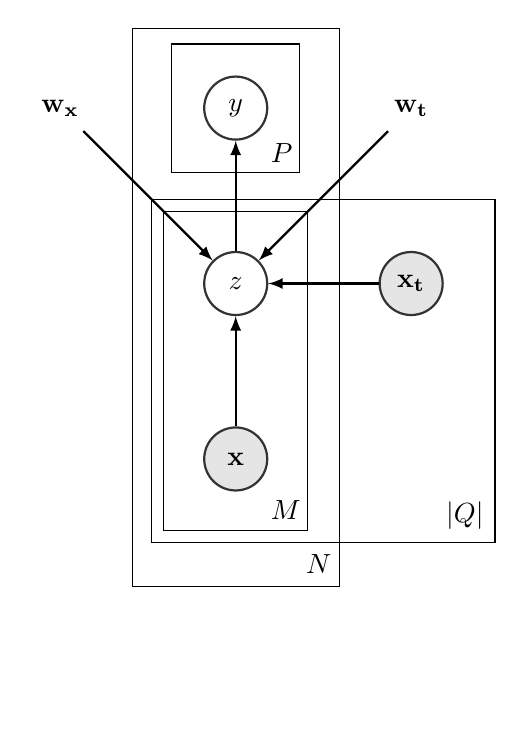
\begin{tikzpicture}
\tikzstyle{main}=[circle, minimum size = 8mm, thick, draw =black!80, node distance = 14mm]
\tikzstyle{mainnob}=[circle, minimum size = 8mm, thick, draw =white!100, node distance = 14mm]
\tikzstyle{connect}=[-latex, thick]
\tikzstyle{box}=[rectangle, draw=black!100]
\node[main, fill = white!100] (y) [label=center:$y$] { };
\node[rectangle, inner sep=-1mm, fit=(y),label=below right:$P$] {};
\node[rectangle, inner sep=4mm, fit=(y),draw=black!100] {};
\node[main, fill = white!100] (z) [below=of y,label=center:$z$] { };
%\node[rectangle, inner sep=-1mm, fit=(z),label=below right:$P$] {};
%\node[rectangle, inner sep=4mm, fit=(z),draw=black!100] {};
\node[main, fill = black!10] (x) [below=of z,label=center:$\mathbf{x}$] { }; 
\node[main, fill = black!10] (t) [right=of z,label=center:$\mathbf{x_t}$] { };
\node[mainnob, fill = white!100] (wt) [right=of y,label=center:$\mathbf{w_t}$] { };
\node[mainnob, fill = white!100] (wx) [left=of y,label=center:$\mathbf{w_x}$] { };
\node[rectangle, inner sep=-1mm, fit=(z)(x)(t),label=below right:$|Q|$, yshift=-1mm] {};
\node[rectangle, inner sep=6.5mm, fit=(z)(x)(t),draw=black!100] {};

\node[rectangle, inner sep=-1mm, fit=(z)(x),label=below right:$M$,yshift=-12mm] {};
\node[rectangle, inner sep=5.0mm, fit=(z)(x),draw=black!100] {};

\node[rectangle, inner sep=-1mm, fit=(x)(z)(y),label=below right:$N$,yshift=-30mm,xshift=4.5mm] {};
\node[rectangle, inner sep=9mm, fit=(x)(z)(y),draw=black!100, yshift=-3mm] {};

\path (wx) edge [connect] (z)
(x) edge [connect] (z)
(z) edge [connect] (y)
(wt) edge [connect] (z)
(t) edge [connect] (z);
\end{tikzpicture}
\vspace{-15mm}
\caption{QnA-based relation extraction model plate diagram.
$N$ - number of different entity pairs, $M$ - number of mentions of an entity pair, $|Q|$ - number of questions where an entity pair is mentioned, $\mathbf{x}$ and $\mathbf{x_t}$ - mention-based and question-based features, $\mathbf{w}$ and $\mathbf{w_t}$ - corresponding feature weights, latent variables $z$ - relation expressed in an entity pair mention, latent variables $y$ - relations between entity pair}
\label{fig:qna_relextract:graphmodel}
\end{figure}

Our models for relation extraction from QnA data incorporates the topic of the question and can be represented as a graphical model (Figure \ref{fig:qna_relextract:graphmodel}).
Each mention of a pair of entities is represented with a set of mention-based features $x$ and question-based features $x_t$.
A multinomial latent variable $z$ represents a relation (or none) expressed in the mention and depends on the features and a set of weights $w_x$ for mention-based and $w_t$ for question-based features:
$$\hat{z}=\argmax{z \in P \cup \emptyset} p(z|x, x_t, w_x, w_t)$$.
To estimate this variable we use L2-regularized multinomial logistic regression model, trained using the distant supervision approach for relation extraction \cite{MintzBSJ09}, in which mentions of entity pairs related in Freebase are treated as positive instances for the corresponding predicates, and negative examples are sampled from mentions of entity pairs which are not related by any of the predicates of interest.
Finally, to predict a set of possible relations $\mathbf{y}$ between the pair of entities we take logical OR of individual mention variables $\mathbf{z}$, \ie $y_p = \lor_{i=1}^M [z_i = p, p \in P]$, where M is the number of mentions of this pair of entities.

\subsubsection{Sentence-based baseline model}

Existing sentence-based relation extraction models can be applied to individual sentences of a QnA pair and will work well for complete statements, \eg ``Who did Brad Pitt marry? Brad Pitt and Angelina Jolie married at secret ceremony''.
In sentence-based scenario, when the set of question-based features is empty, the above model corresponds to the Mintz++ baseline described in \cite{Surdeanu:2012:MML:2390948.2391003}, which was shown to be superior to the original model of \cite{MintzBSJ09}, is easier to train than some other state of the art distant supervision models and produces comparable results.

\subsubsection{Sentence-based model with question features}

\begin{table*}[tbh]
\centering
\caption{Examples of features used for relation extraction for ``\emph{When was Mariah Carey born? Mariah Carey was born 27 March 1970}''}
\vspace{-2mm}
\label{table:qna_relextract:features}
\begin{tabular}{|p{8cm}|p{8cm}|}
\hline
\multicolumn{2}{|c|}{Sentence-based model}\\
\hline
Dependency path between entities & [PERSON]$\rightarrow$nsubjpass(born)tmod$\leftarrow$[DATE]\\
Surface pattern & [PERSON] be/VBD born/VBN [DATE]\\
\hline
\hline
\multicolumn{2}{|c|}{Question features for sentence-based model}\\
\hline
Question template & when [PERSON] born\\
Dependecy path from a verb to the question word & (when)$\rightarrow$advmod(born)\\
Question word + dependency tree root & when+born\\
\hline
\hline
\multicolumn{2}{|c|}{QnA-based model}\\
\hline
Question template + answer entity type & Q: when [PERSON] born A:[DATE]\\
Dependency path from question word to entity & Q:(when)$\rightarrow$advmod(born)nsubj$\leftarrow$[PERSON]\\
and answer entity to the answer tree root & A: (born)tmod$\leftarrow$[DATE]\\
Question word, dependency root and answer pattern & Q: when+born A:born [DATE]\\
\hline
\end{tabular}
\end{table*}

In many cases an answer statement is hard to interpret correctly without knowing the corresponding question.
To give the baseline model some knowledge about the question, we include question features (Table \ref{table:qna_relextract:features}), which are based on dependency tree and surface patterns of a question sentence. 
This information can help the model to account for the question topic and improve predictions in some ambiguous situations.

\subsubsection{QnA-based model}
The QnA model for relation extraction is inspired by the observation, that often an answer sentence do not mention one of the entities at all, \eg, ``\textit{When was Isaac Newton born? December 25, 1642 Woolsthorpe, England}''.
To tackle this situation we make the following assumption about the discourse of a QnA pair: an entity mentioned in a question is related to entities in the corresponding answer and the context of both mentions can be used to infer the relation predicate.
Our QnA-based relation extraction model takes an entity from a question sentence and entity from the answer as a candidate relation mention, represents it with a set features (Table \ref{table:qna_relextract:features}) and predicts a possible relation between them similar to sentence-based models.
The features are conjunctions of various dependency tree and surface patterns of question and answer sentences, designed to capture their topics and relation.

\subsubsection{Experiments}

For experiments we used 2 publicly available CQA datasets: Yahoo! Answers WebScope dataset\footnote{http://webscope.sandbox.yahoo.com/catalog.php?datatype=l} and a crawl of WikiAnswers\footnote{http://wiki.answers.com/} collected by \cite{Fader:2014:OQA:2623330.2623677}.
The Yahoo! Answers dataset contains 4,483,032 questions (3,894,644 in English) with the corresponding answers collected on 10/25/2007.
The crawl of WikiAnswers has 30,370,994 question clusters, tagged by WikiAnswers users as paraphrases, and only 3,386,256 them have answers.
From these clusters we used all possible pairs of questions and corresponding answers (19,629,443 pairs in total).

\begin{table*}[ht]
\centering
\caption{Yahoo! Answers and WikiAnswers datasets statistics}
\vspace{-2mm}
\label{table:qna_relextract:cqastats}
\begin{tabular}{|p{12.5cm}||p{1.2cm}|p{1.2cm}|} \hline
& Y!A & WA\\
\hline
Number of QnA pairs & 3.8M & 19.6M \\
Average question length (in chars) & 56.67 & 47.03 \\
Average answer length (in chars) & 335.82 & 24.24 \\
% Number of resolved entities per QnA pair & 3.57 & 3.23 \\
Percent of QnA pairs with answers that do not have any verbs & 8.8\% & 18.9\% \\
Percent of QnA pairs with at least one pair of entities related in Freebase & 11.7\% & 27.5\% \\
Percent of relations between entity pairs in question sentences only & 1.6 \% & 3.1\% \\
Percent of relations between entity pairs in question and answer sentences only & 28.1\% & 46.4\% \\
Percent of relations between entity pairs in answer sentences only & 38.6\%& 12.0\%\\
\hline
\end{tabular}
\end{table*}

For each QnA pair we applied tokenization, sentence detection, named entity tagger, parsing and coreference resolution from Stanford CoreNLP \cite{manning-EtAl:2014:P14-5}.
Our cascade entity linking approach is similar to \cite{chang2011stanford} and considered all noun phrase and named entity mentions as candidates.
First all named entity mentions are looked up in Freebase names and aliases dictionary.
The next two stages attempt to match mention text with dictionary of English Wikipedia concepts \cite{spitkovsky2012cross} and its normalized version.
Finally for named entity mentions we try spelling correction using Freebase entity names dictionary.
We didn't disambiguate entities and instead took top-5 ids for each coreference cluster (using the $p(entity|phrase)$ score from the dictionary or number of existing Freebase triples).
All pairs of entities (or entity and date) in a QnA pair that are directly related\footnote{We also consider some paths that come through a mediator node, \eg  /people/person/spouse\_s./people/marriage/spouse} in Freebase were annotated with the corresponding relations.

Table \ref{table:qna_relextract:cqastats} gives some statistics on the datasets used in this work.
The analysis of answers that do not have any verbs show that $\sim$8.8\% of all QnA pairs do not state the predicate in the answer text.
The percentage is higher for WikiAnswers, which has shorter answers on average.
Unfortunately, for many QnA pairs we were unable to find relations between the mentioned entities (for many of them no or few entities were resolved to Freebase).
Among those QnA pairs, where some relation was annotated, we looked at the location of related entities.
In Yahoo! Answers dataset 38.6\% (12.0\% for WikiAnswers) of related entities are mentioned in answer sentences and can potentially be extracted by sentence-based model, and 28.1\% (46.4\% for WikiAnswers) between entities mentioned in question and answer sentences, which are not available to the baseline model and our goal is to extract some of them.

For our experiments we use a subset of 29 Freebase predicates that have enough unique instances annotated in our corpus, \eg date of birth, profession, nationality, education institution, date of death, disease symptoms and treatments, book author, artist album, \etc
We train and test the models on each dataset separately.
Each corpus is randomly split for training (75\%) and testing (25\%).
Knowledge base facts are also split into training and testing sets (50\% each).
QnA and sentence-based models predict labels for each entity pair mention, and we aggregate mention predictions by taking the maximum score for each predicate.
We do the same aggregation to produce a combination of QnA- and sentence-based models, \ie, all extractions produced by the models are combined and if there are multiple extractions of the same fact we take the maximum score as the final confidence.
The precision and recall of extractions are evaluated on a test set of Freebase triples, \ie an extracted triple is considered correct if it belongs to the test set of Freebase triples, which are not used for training (triples used for training are simply ignored).
Note, that this only provides a lower bound on the model performance as some of the predicted facts can be correct and simply missing in Freebase.

Figure \ref{fig:qna_relextract:pr_curve} shows Precision-Recall curves for QnA-based and sentence-based baseline models and some numeric results are given in Table \ref{table:qna_relextract:results}.
As 100\% recall we took all pairs of entities that can be extracted by either model.
It is important to note, that since some entity pairs occur exclusively inside the answer sentences and some in pairs of question and answer sentences, none of the individual models is capable of achieving 100\% recall, and maximum possible recalls for QnA- and sentence-based models are different.

\begin{figure}[h!]
\centering
\vspace{-2mm}
\begin{subfigure}[h]{0.45\textwidth}
	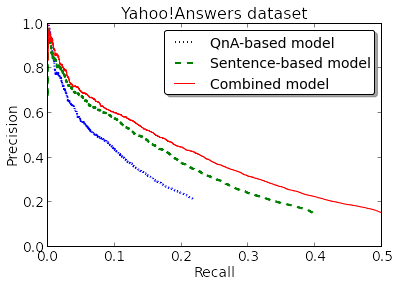
\includegraphics[width=0.99\textwidth]{img/qa_vs_sent_ya}
	\vspace{-1mm}
    \label{figure:pr:ya}
\end{subfigure}
\begin{subfigure}[h]{0.45\textwidth}
	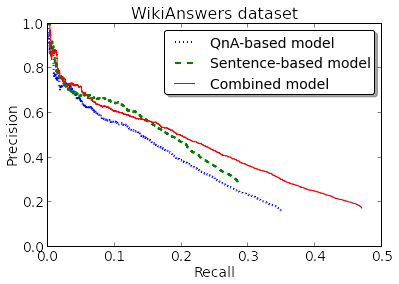
\includegraphics[width=0.99\textwidth]{img/qa_vs_sent_wa}
	\vspace{-1mm}
    \label{figure:pr:wa}
\end{subfigure}
\begin{subfigure}[h]{0.45\textwidth}
	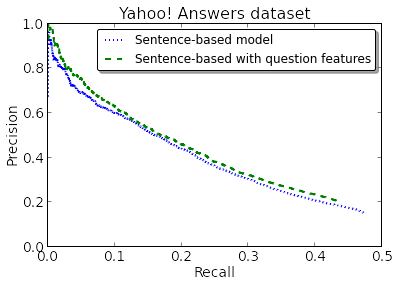
\includegraphics[width=0.99\textwidth]{img/noqf_vs_qf}
	\vspace{-1mm}
	\label{figure:pr:noqf_vs_qf}
\end{subfigure}
\vspace{-1mm}
\caption{Precision-Recall curves for QnA-based vs sentence-based models and sentence-based model with and without question features}
\label{fig:qna_relextract:pr_curve}
\end{figure}

\begin{table*}[tbh]
\centering
\caption{Extraction results for QnA- and sentence-based models on both datasets}
\vspace{-2mm}
\label{table:qna_relextract:results}
\begin{tabular}{|p{6.6cm}||p{0.9cm}|p{1.4cm}|p{1.6cm}||p{0.9cm}|p{1.4cm}|p{1.6cm}|}
\hline
& \multicolumn{3}{|c||}{Yahoo! Answers} & \multicolumn{3}{|c|}{WikiAnswers}\\
\cline{2-7}
& QnA & Sentence & Combined & QnA & Sentence & Combined\\
\hline
F-1 score & 0.219 & 0.276 & 0.310 & 0.277 & 0.297 & 0.332\\
Number of correct extractions & 3229 & 5900 & 7428 & 2804 & 2288 & 3779 \\
Correct triples not extracted by other model & 20.5\% & 56.5\% & - & 39.4\% & 25.8\% & - \\
\hline
\end{tabular}
\end{table*}

Results demonstrate that from 20.5\% to 39.4\% of correct triples extracted by the QnA-based model are not extracted by the baseline model, and the combination of both models is able to achieve higher precision and recall.
Unfortunately, comparison of sentence-based model with and without question-based features (Figure \ref{fig:qna_relextract:pr_curve}) didn't show a significant difference.

\subsubsection{Analysis}

To get an idea of typical problems of QnA-based model we sampled and manually judged extracted high confidence examples that are not present in Freebase (and thus are considered incorrect for precision-recall analysis).

The major reason (40\%) of false positive extractions is errors in entity linking.
For example: ``\emph{Who is Tim O'Brien? He was born in Austin on October 1, 1946}''.
The model was able to correctly extract [Tim O'Brien, date\_of\_birth, October 1, 1946], however Tim O'Brien was linked to a wrong person.
In a number of cases (16\%) our discourse model turns out to be too simple and fails for answers, that mention numerous additional information, \eg ``\emph{How old is Madonna really? ...Cher was born on 20 May 1946 which makes her older that Madonna...}''.
A possible solution would be to either restrict QnA-based model to cases when no additional information is present or design a better discourse model with deeper analysis of the answer sentence and its predicates and arguments.
Some mistakes are due to distant supervision errors, for example for the music.composition.composer predicate our model extracts singers as well as composers (which are in many cases the same).

Of course, there are a number of cases, when our extractions are indeed correct, but are either missing (33\%) or contradicting with Freebase (8\%).
An example of an extracted fact, that is missing in Freebase is ``\emph{Who is Wole Soyinka? He studied at the University College, Ibadan(1952-1954) and the University of Leeds (1954-1957)}'', and [Wole Soyinka, institution, University of Leeds] is currently not present in Freebase.
Contradictions with Freebase occur because of different precision levels (``pianist'' vs ``jazz pianist'', city vs county, \etc), different calendars used for dates or ``incorrect'' information provided by the user.
An example, when existing and extracted relation instance are different in precision is:``\emph{Who is Edward Van Vleck? Edward Van Vleck was a mathematician born in Middletown, Connecticut}'' we extract [Edward Van Vleck, place\_of\_birth, Middletown], however the Freebase currently has USA as his place of birth.

The problem of ``incorrect'' information provided in the answer is very interesting and worth special attention.
It has been studied in CQA research, \eg \cite{shah2010evaluating}, and an example of such QnA pair is: ``\emph{Who is Chandrababu Naidu? Nara Chandra Babu Naidu (born April 20, 1951)}''.
Other authoritative resources on the Web give April 20, 1950 as Chandrababu Naidu's date of birth.
This raises a question of trust to the provided answer and expertise of the answerer.
Many questions on CQA websites belong to the medical domain, \eg people asking advices on different health related topics.
How much we can trust the answers provided to extract them into the knowledge base?
We leave this question to the future work.

Finally, we have seen that only a small fraction of available QnA pairs were annotated with existing Freebase relations, which shows a possible limitation of Freebase schema.
A promising direction for future work is automatic extraction of new predicates, which users are interested in and which can be useful to answer more future questions.

\subsubsection{Conclusion}

In this section we described a model for relation extraction from QnA data, which is capable of predicting relations between entities mentioned in question and answer sentences.
We conducted experiments on 2 publicly available CQA datasets and showed that our model can extract triples not available to existing sentence-based techniques and can be effectively combined with them for better coverage of a knowledge base population system.


% BELOW IS MY ANOTHER IDEA, BUT IT'S VAGUE AND DOESN'T HAVE ANY CONCRETE PLAN
% \subsection{Question-guided relation extraction}
%\label{subsec:question_based_relextract}
%The idea is that we can aggregate related questions and relation extraction patterns.
%When a person asks a question, we retrieve passages and sentences to extract the answer from.
%Imaging a question is asking a certain property of an entity.
%If we can retrieve a sentence, that mentions this entity along with a candidate answer, we can build a pattern for relation extraction.
%This pattern will be connected to the question ``template''.
%Likewise, if we already have relation extraction patterns we can boost those that are retrieve in response to the question and save this connection.

%Hypothesis:
%\begin{enumerate}
%\item Patterns retrieved in response to the question are better in quality, we can boost them. We can try to verify this on some relation extraction dataset and questions from some query log. We can also try to use some KBQA dataset.
%\item Patterns mined for questions should help question answering. This is essentially weak supervision for training knowledge base question answering using text based question answering.
%\end{enumerate}

%Problems:
%\begin{itemize}
%\item How to extract new predicates? If we have a question, and a sentence is mentioning a pair of non-related entities, how can we make a new one?
%\item How to deal with more complex questions, that are not simple relations
%\end{itemize}

%Useful dataset: MSN query log, SimpleQuestions from Facebook, WebQuestions, NYT relation extraction dataset.

%This approach can also be applied to open IE.
%There are sentence selection methods for question answering.
%We can extract noun phrases (NP mentioned in question and supposedly answer NP), and then aggregate all sentences, that mention the same NPs together.
%Hypothesis is, that we can extract patterns, that will answer the same question for other entities.

% =-=-=-=-=-=-=-=-=-=-=-=-=-=-=-=-=-=-=-=-=-=-=-=-=-=-=-=-=-=-=-=-=-=-=-=-=-

\section{Semantic Text Annotations for Hybrid Question Answering}
\label{sec:text+kb}

Converting unstructured information into structured form by extracting knowledge from text suffers from certain quality losses.
Existing relation extraction tools aren't perfect, in particular due to recall losses a lot of information is left behind.
Moreover, extractions contain certain level of incorrect information due to precision losses.
These errors cap the upper bound on the question answering system performance.

Here I propose to utilize the synergy of structured and unstructured data, and exploit the advantages of each of them to overcome the limitations of the other.
More particularly, I propose to annotate and index mentions of knowledge base entities in text documents, which essentially induce a special kind of edges to the knowledge base, and allows one to traverse these edges in both directions.
These links open up many opportunities for QA reasoning, \eg retrieving all the information about the entity by going from a mention to a KB entity, finding relations between entities by retrieving text passages that mention both of them, extracting candidate evidence by retrieving passages that mention question and answer entities along with some question terms, and so on.
First, in Section \ref{subsec:text2kb} we describe how external text data can help to improve the performance of knowledge base question answering, and in Section \ref{subsec:text+kb} I propose a novel hybrid question answering architecture.

\subsection{Text2KB: Knowledge Base Question Answering using External Text Data}
\label{subsec:text2kb}

We now introduce our system, called Text2KB, that expands upon the basic KBQA model by incorporating external textual sources throughout the QA process. The general architecture and an example use case of Text2KB is presented on Figure \ref{fig:text2kb:model}. 
The left part of the figure roughly corresponds to the architecture of the existing information extraction approaches to KBQA, described above.
The right part introduces additional external text data sources, specifically
we investigate the use of web search results, community question answering (CQA) data, and a large collection of documents with detected KB entity mentions.
Recall that the main challenges in KBQA are linking topical entities in the question to the KB; identifying candidate answers in the neighborhood around the question entities; and ranking the candidates. In the rest of this section we present our approach to solving each of these challenges, by: using web search results, CQA data, and external corpus statistics. 

\begin{figure}[h]
\centering
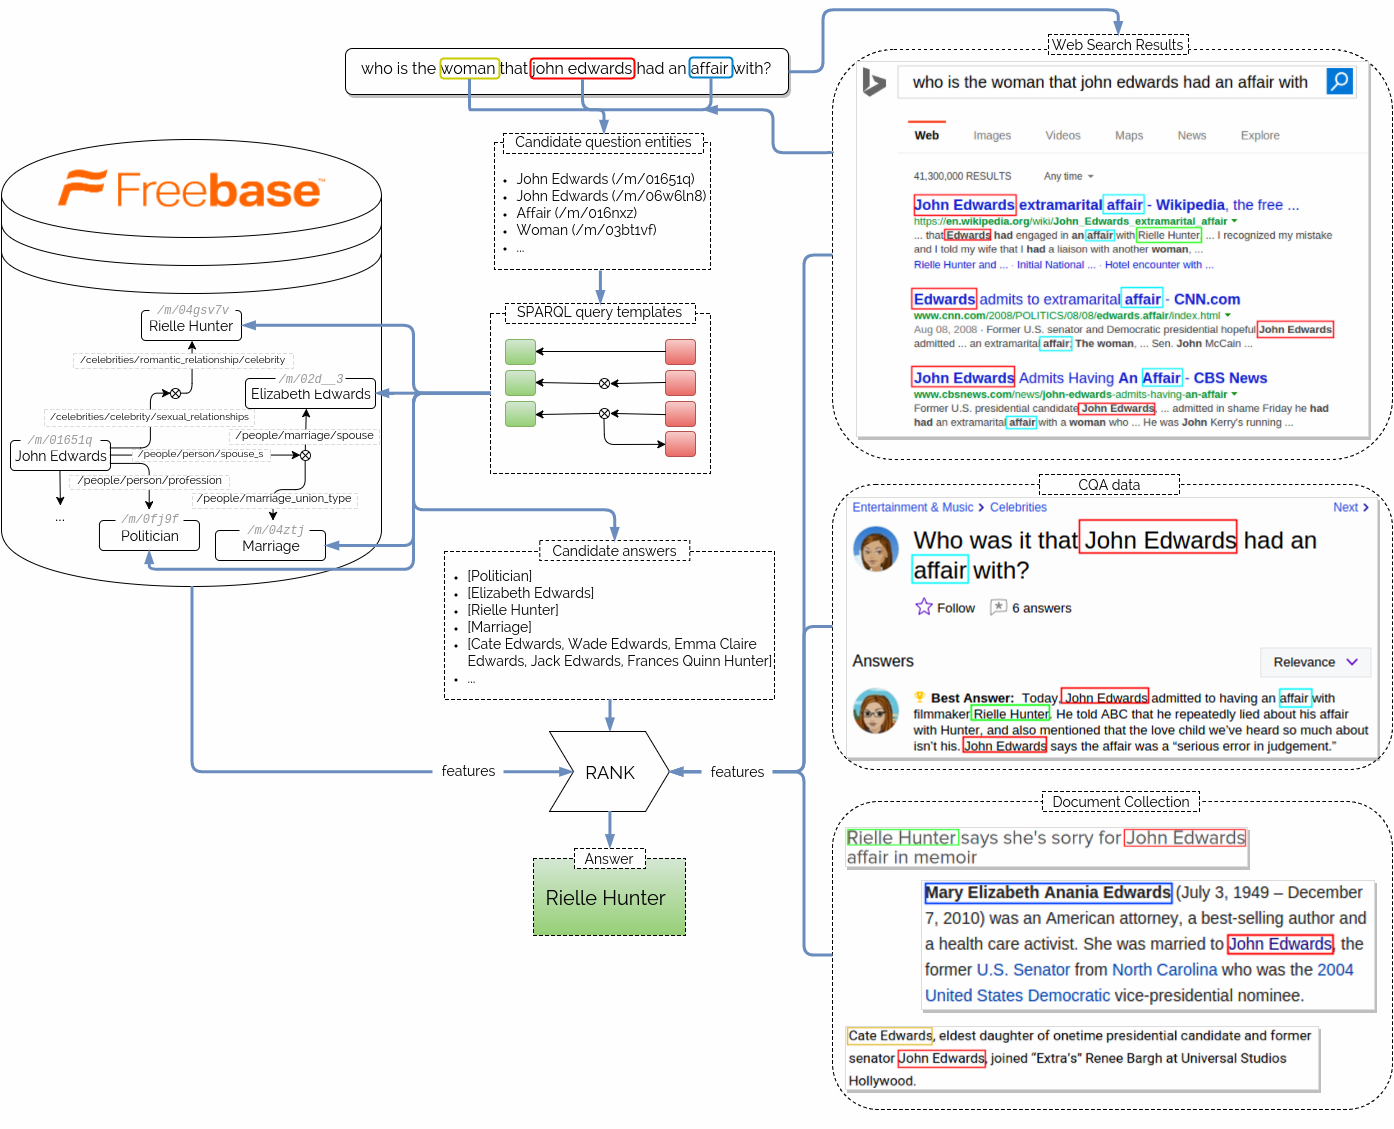
\includegraphics[width=1.0\textwidth]{img/Text2KB_model}
\caption{The architecture of our Text2KB Question Answering system}
\label{fig:text2kb:model}
\end{figure}

\subsubsection{Web search results for KBQA}
\label{subsubsec:text2kb:method:web}

To obtain related web search results, Text2KB issues the question as a query to a commercial web search engine\footnote{https://datamarket.azure.com/dataset/bing/search}, extracts top 10 search result snippets and the corresponding documents.
Next, it detects KB entity mentions in both snippets and documents.
% Document snippets are usually built to present the information most relevant to the query, and often contain answers to a question.
% Unfortunately, for longer queries the snippets often represent and combination of small phrases, that contain mostly question terms and very few additional information.
% Nevertheless, we keep both snippets and documents text, and using thesystem's linker detect KB entity mentions.
This data turns out to be useful for multiple purposes, \ie question entity identification and answer candidate ranking.

\textbf{Question entity identification}.
Question text provides only a limited context for entity disambiguation and linking; additionally, the entity name can be misspelled or an uncommon variation used.
This complicates the task of entity identification, which is the foundation of whole question answering process.
Fortunately, web search results help with these problems, as they usually contain multiple mentions of the same entities and provide more context for disambiguation.
Text2KB uses the search result snippets to {\em expand} the set of detected question entities.
To keep only the entities that are also mentioned in the question and avoid irrelevant entities, we use string distance.
More specifically, we take names of all entities detected in the question and compute their term by term similarity with non-stopwords from the question.
In this work we used Jaro-Winkler string distance and entity was added to the list of question entities if at least one of its tokens $e_t$ has high similarity with one of the question tokens $q_t$ excluding stopwords ($Stop$):
$$max_{e_t \in M\backslash Stop, q_t \in Q\backslash Stop} distance_{Jaro-Winkler}(e_t, q_t) \geq 0.8$$

\textbf{Answer candidate features}.
Most of the information stored in knowledge bases is also present in other formats, including natural language statements, tables, \etc
For example, on Figure \ref{fig:text2kb:web_search_entitylink} multiple snippets mention the date when Tutankhamun became the king.
Text-QA systems usually generate answer candidates from passages extracted from retrieved documents.
In our case candidates are already generated from a KB and we just need to rank them to select the best one.
Text2KB uses snippets and documents to compute a set of features, which are used for answer candidate ranking.
More specifically we do this following:

\begin{figure}[h]
\centering
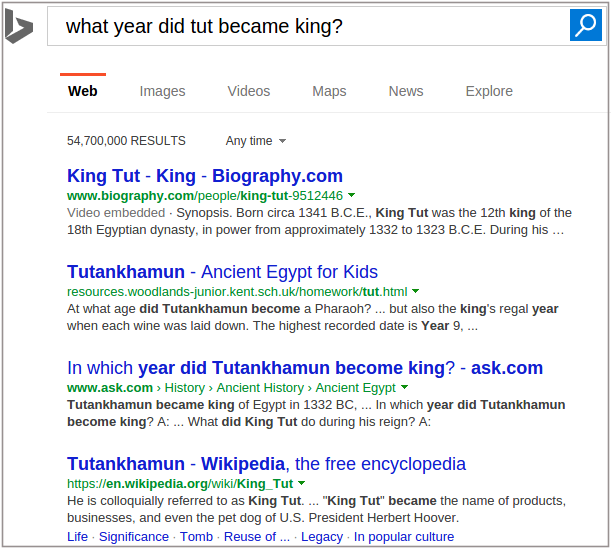
\includegraphics[width=0.5\textwidth]{img/web_search_entitylink}
\caption{Search results for the question \textit{``what year did tut became king?''}, which mention both the full name of the king and the correct answer to the question}
\label{fig:text2kb:web_search_entitylink}
\end{figure}

\begin{enumerate}
\setlength\itemsep{-0.5em}
\item Precompute term and entity IDFs\footnote{https://en.wikipedia.org/wiki/Tf-idf}. We used Google n-grams corpus to approximate terms IDF by collection frequencies and available ClueWeb Freebase entity annotations\footnote{http://lemurproject.org/clueweb09/FACC1/} to compute entity IDFs
\item Each snippet and document is represented by two TF-IDF vectors of lowercased tokens and mentioned entities
\item In addition, vectors of all snippets and all documents are merged together to form combined token and entity vectors
\item Each answer candidate is also represented as TF-IDF vectors of terms (from entity names) and entities
\item We compute cosine similarities between answer and each snippet and document token and entity vectors. This gives us 10 similarity scores for every document for token vectors and 10 similarities for entity vectors, we take average and maximum scores as features.
\item We do the same for the combined document and use cosine similarities as features.
\end{enumerate}

\subsubsection{CQA data for Matching Questions to Predicates}
\label{subsubsec:text2kb:method:cqa}

Recall that a major challenge in KBQA is that natural language questions do not easily or uniquely map to entities and predicates in a KB. An established approach for this task is supervised machine learning, which requires labeled examples of questions and the corresponding answer to learn this mapping. Unfortunately, manual labeling of questions with answers is expensive, and necessarily contains only a small fraction of the different ways the same KB predicate can be inquired about using natural language questions. Researchers have proposed to use weakly supervised methods to extend the lexicon with mappings learned from \textit{single sentence statements} mentioning entity pairs from a large corpus \cite{YaoD14}.
However, often there is a lexical gap between how information is asked about in a question and how it is expressed in a statement.
On the other hand there are huge archives of questions and answers posted by real users on various community question answering websites, \eg Figure \ref{fig:text2kb:cqa_example}.

\begin{figure}
\centering
\fbox{
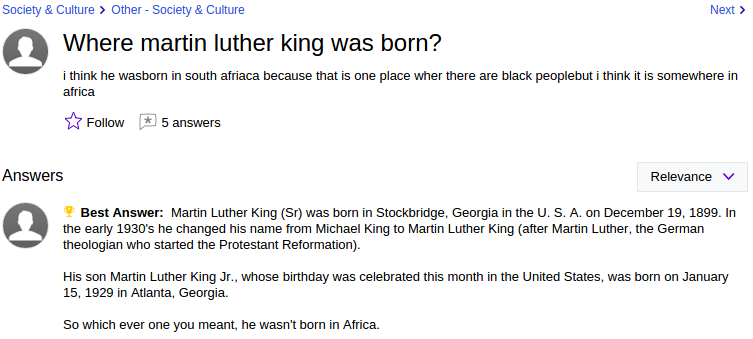
\includegraphics[width=0.5\textwidth]{img/cqa_example}
}
\caption{Example of a question and answer pair from Yahoo! Answers CQA website}
\label{fig:text2kb:cqa_example}
\end{figure}

For our experiments we use 4,483,032 questions from Yahoo! Comprehensive Questions and Answers WebScope dataset\footnote{https://webscope.sandbox.yahoo.com/catalog.php?datatype=l}.
Texts of each question and answer pair were run through an entity linker, that detected mentions of Freebase entities.
Next, similar to an idea of relation extraction from CQA data \cite{savenkov2015relation}, we use distant supervision to label each question-answer pair with predicates between entities mentioned in the question and in the answer.
As a result, we have a set of questions, annotated with KB predicates, which are, often incorrectly, assumed to answer the question.
We learn the associations between question terms and predicates by computing pointwise mutual information scores\footnote{https://en.wikipedia.org/wiki/Pointwise\_mutual\_information} (PMI) for each term-predicate pair.
Examples of scores for some terms from WebQuestions dataset questions are given in Table \ref{table:text2kb:cqa_npmi}.

\begin{table}
\centering
\caption{Examples of term-predicate pairs with high PMI scores, computed using distant supervision from a CQA collection}
\label{table:text2kb:cqa_npmi}
\begin{tabular}{| p{2cm} | p{8cm} | p{2cm} |}
\hline
Term & Predicate & PMI score\\
\hline
born & people.person.date\_of\_birth & 3.67\\
 & people.person.date\_of\_death & 2.73\\
 & location.location.people\_born\_here & 1.60\\
\hline
kill & people.deceased\_person.cause\_of\_death & 1.70\\
& book.book.characters & 1.55\\
\hline
currency & location.country.currency\_formerly\_used & 5.55 \\
& location.country.currency\_used & 3.54 \\
\hline
school & education.school.school\_district & 4.14 \\
& people.education.institution & 1.70\\
& sports.school\_sports\_team.school & 1.69 \\
\hline
illness & medicine.symptom.symptom\_of & 2.11\\
& medicine.decease.causes & 1.68\\
& medicine.disease.treatments & 1.59\\
\hline
win & sports.sports\_team.championships & 4.11\\
& sports.sports\_league.championship & 3.79\\
\hline
\end{tabular}
\end{table}

Although noisy, the statistics look reasonable to be used for candidate ranking.
In Text2KB we take candidate answer predicates and look up the  PMI scores between these predicates and terms in the question.
Missing pairs are given a score of 0, and minimum, average and maximum of these scores are used as features.
Since this kind of data is usually sparse, we also use pretrained word2vec word embeddings\footnote{https://code.google.com/p/word2vec/} to generate predicate embeddings by taking weighted average of term vectors from predicate's PMI table.
Each term's embedding vector is weighted by its PMI value (terms with negative score are skipped).
Then, we compute cosine similarities between predicate vector and question term vectors and take their minimum, average, maximum as features.
Similarity between the predicate vector and average question term vector is also computed.


\subsubsection{Estimating Entity Associations}
\label{subsubsec:text2kb:method:clueweb}

When ranking candidate answers, we are interested in estimating whether the entities in the question and the answer are related in a way asked in the question.
Existing systems usually look on how candidate predicates are expressed in questions and statements.
But predicate isn't the only way we can look at this. An alternative is to consider text passages, \eg sentences, that mention topical and answer entities together.
For example, in the bottom right corner of Figure \ref{fig:text2kb:model} we can see some passages that mentioned a pair of people, and the context of these mentions often expresses the nature of the relationships between the entities.

We use the ClueWeb12 corpus with existing Freebase entity annotations\footnote{http://lemurproject.org/clueweb12/FACC1/} and compute counts of different terms that occur in the context to an entity pair mention.
By an entity pair mention we mean a pair of mentions of different entities within 200 characters of each other.
We take terms in between mentions and 100 character before and after mentions as the context.
A small sample of this data is presented in Table \ref{table:text2kb:clueweb_entitypairs_langmodel}.

\begin{table}
\centering
\caption{Example of entity pairs along with the most popular terms mentioned around the entities}
\label{table:text2kb:clueweb_entitypairs_langmodel}
\begin{tabular}{| p{4cm} | p{4cm} | p{8cm} |}
\hline
Entity 1 & Entity 2 & Term counts\\
\hline
John Edwards & Rielle Hunter & campaign, affair, mistress, child, former ...\\
\hline
John Edwards & Cate Edwards & daughter, former, senator, courthouse, left, greensboro, eldest ...\\
\hline
John Edwards & Elizabeth Edwards & wife, hunter, campaign, affair, cancer, rielle, husband ...\\
\hline
John Edwards & Frances Quinn Hunter & daughter, john, rielle, father, child, former, paternity...\\
\hline
\end{tabular}
\end{table}

First, given a set of question terms $Q$ and an answer candidate, that starts from a question entity $e_1$, we compute a language model score for every answer entity $e_2$:
$$p(Q|e_1, e_2) = \prod_{t\in Q} p(t | e_1, e_2)$$
and use minimum, average and maximum as features.
To address the sparsity problem, we again use embeddings, 
ie for each entity pair a weighted (by counts) average embedding vector of terms is computed and minimum, average and maximum cosine similarities between these vectors and question tokens vector are used as features.

\subsubsection{Internal text data to enrich entity representation}
\label{subsubsec:text2kb:internal_text}

In addition to external text data, many knowledge bases, including Freebase, contain text data as well.
In Freebase, most of the entities contain a description paragraph, which often comes from the entity Wikipedia profile.
These descriptions of entities in the KB were found useful for text-based question answering \cite{Sun:2015:ODQ:2736277.2741651}.
For completeness, we include them in our system. The aim is to improve the matching of the question text, to the unstructured description of the candidate entities. For this, each entity description is represented as a vector of tokens, and a vector of mentioned entities. We compute cosine similarities between the question tokens and each of the candidate entity vectors, and use these scores as features for candidate ranking.
In future work, we could explore incorporating any other entity profile text, such as full Wikipedia article.


\subsubsection{Evaluation}
\label{subsubsec:text2kb:evaluation}

We followed the standard evaluation procedure for the WebQuestions dataset and used the original 70-30\% train-test split, which results in 3,778 training and 2,032 test questions.
Since each answer is potentially a list of entities $a^*$, the quality of an answer $a$ is represented by F1-score: 
$$f1(a^*, a) = 2\frac{precision(a^*,a) recall(a^*,a)}{precision(a^*,a) + recall(a^*,a)}$$
where $precision(a^*, a)=\frac{|a^* \cap a|}{|a|}$ and $recall(a^*, a) = \frac{|a^* \cap a|}{|a^*|}$.

We also report average precision and recall, as well as an F1 score of average precision and recall.
The results of existing approaches, our baseline and Text2KB systems is presented in Table \ref{table:text2kb:webquestions_results}.

\begin{table}
\centering
\caption{Performance of the Text2KB system on WebQuestions dataset compared to the existing approaches. The difference from the baseline Aqqu system is significant with p-value < 0.01}
\label{table:text2kb:webquestions_results}
\begin{tabular}{| p{5cm} | p{1.5cm} | p{1.5cm} | p{1.5cm} | p{1.5cm} | }
\hline
System & avg Recall & avg Precision & F1 of avg Prec and Recall & avg F1 \\
\hline
SemPre \cite{BerantCFL13:sempre} & 0.413 & 0.480 & 0.444 & 0.357\\
Subgraph Embeddings \cite{BordesCW14:emnlp} & - & - & 0.432 & 0.392\\
ParaSemPre \cite{BerantL14:parasempre} & 0.466 & 0.405 & 0.433 & 0.399\\
Jacana \cite{YaoD14} & 0.458 & 0.517 & 0.486 & 0.330\\
Kitt AI \cite{yao-scratch-qa-naacl2015} & 0.545 & 0.526 & 0.535 & 0.443\\
AgendaIL \cite{berant2015imitation} & 0.557 & 0.505 & 0.530 & 0.497\\
STAGG \cite{yih:ACL:2015:STAGG} & 0.607 & \textbf{0.528} & \textbf{0.565} & \textbf{0.525}\\
% STAGG (no duplicates\footnote{An answer of the STAGG system may contain duplicate entities, which are double counted by the evaluation script}) \cite{yih2015semantic} & 0.6067 & 0.5263 & 0.5634 & 0.5234 \\
\hline
Aqqu (baseline) \cite{bastmore:cikm:2015:aquu} & 0.604 & 0.498 & 0.546 & 0.494\\
% DIDN'T HAVE TIME TO IMPLEMENT THIS.
% Text-only baseline & & & & \\
Our system: Text2KB & \textbf{0.6354} & 0.5059 & 0.5633 & 0.5223 \\
\hline
\end{tabular}
\end{table}

As we can see, Text2KB significantly improves over the baseline system and reaches the current best published result - STAGG \cite{yih:ACL:2015:STAGG}, and we believe that this system will also benefit from the ideas of our work, and we will explore this question in Section \ref{section:text2kb:analysis}.

\textbf{Ablation Study}.
To study effects of different components in isolation we made a series of ablation studies.
For convenience, we introduce the following notations for different components of our system:
\begin{itemize}
\setlength\itemsep{-0.5em}
\item T - notable type score model as a ranking feature
\item DF - date range filter-based query template
% \item TF - using notable type based filter
\item E - using web search result snippets for question entity identification
\item W - using web search results for feature generation
\item CQA - using CQA-based \texttt{[question term, KB predicate]} PMI scores for feature generation
\item CW - features, computed from entity pairs language model, estimated on ClueWeb
\end{itemize}

In our results table we will use the notation \texttt{+$<$component$>$} to for a system with a certain component added, and \texttt{-$<$component$>$} when the component is removed.
For example, the baseline system will be denoted as ``\texttt{Aqqu}'' according the authors notation.
The same system with additional date range filter query templates and notable types score model is denoted as ``\texttt{Aqqu +DF+T}'', which represents the same system as ``\texttt{Text2KB -E-W-CQA-CL}''.
Our full system ``\texttt{Text2KB}'' can be also denoted as ``\texttt{Aqqu +DF+T+E+W+CQA+CL}''.

\begin{table}
\centering
\caption{Average Recall (R), Precision (Pr), and F1 of Aqqu (baseline), Text2KB (our system), and variations of TextKB with respective components removed. * indicates significant differences at p<0.05. }
\label{table:text2kb:ablation:entities_vs_features}
\begin{tabular}{| p{7cm} | c | c | c | }
\hline
System & R & Pr & F1 \\
\hline
% THIS TELLS HOW MUCH EXTERNAL ENTITIES GIVE COMPARED TO MY OTHER IMPROVEMENTS
\texttt{Aqqu} (baseline) & 0.604 & 0.498 & 0.494\\
% baseline_typemodel_dates.log : baseline with types model +dates, but without any text-based data
\texttt{Text2KB -E-W-CQA-CL}=\texttt{Aqqu +DF+T} & 0.6169 & 0.4807 & 0.4987 \\
% extent_dates_typemodel_rf100.log : -web-cqa-clueweb
\texttt{Text2KB -W-CQA-CL} & 0.6272* & 0.4920* & 0.5083* \\  % AND FEATURES GIVE THE REST
% web_cqa_clueweb_typemodel_dates.log : -external entities (Text features on top my other improvements)
\texttt{Text2KB -E} & 0.6344* & 0.4966* & 0.5140* \\  % AND FEATURES GIVE THE REST
%\hline
% extent_web_cqa_clueweb_dates_types_typemodel_rf100.log : everything, including type filters
%\texttt{Text2KB} & 0.6354* & 0.5059* & 0.5223* \\
\hline
\end{tabular}
\end{table}

The first question that we are asking is what are the improvements, introduced by adding date range filter templates, notable type model, entity linking from web search results and text-based features generated from all the different sources.
Results of this ablation experiment are presented in Table \ref{table:text2kb:ablation:entities_vs_features}.
As we can see, additional date range filters and notable types model (\texttt{Text2KB -E-W-CQA-CL}) are responsible for an increased recall and a drop in precision compared to the baseline model.
Detecting question entities (\texttt{Text2KB -W-CQA-CL}) help improve both precision and recall, and therefore average F1 score by 0.096 points.
An even bigger improvement is achieved by introducing all our external text-based features, and since these improvements are independent, their combination boosts the performance even more.

Now, let's look into the relative importance of each of the data sources, we will remove or use a group of web search, cqa or clueweb-based features and see how the performance of the whole system changes.
Table \ref{table:text2kb:ablation:features} summarizes the results of these experiments.

\begin{table}
\centering
\caption{Average Recall (R), Precision (Pr), and F1 of Text2KB variations with and without features based on web search results, CQA data and ClueWeb collection}
\label{table:text2kb:ablation:features}
\begin{tabular}{| p{7cm} | c | c | c | }
\hline
System & R & Pr &  F1 \\
\hline
% THIS PART ANSWERS HOW GOOD ARE EACH OF THE PROPOSED DATASETS
% extent_cqa_clueweb_dates_typemodel_rf100.log : -web
\texttt{Text2KB -W} & 0.6327 & 0.4960 & 0.5126 \\
% extent_web_clueweb_dates_typemodel_rf100.log : -cqa
\texttt{Text2KB -CQA} & 0.6420 & 0.4987 & 0.5185 \\
% extent_web_cqa_dates_typemodel_rf100.log : -clueweb
\texttt{Text2KB -CL} & 0.6444 & 0.5047 & 0.5228 \\
\hline
% extent_web_dates_typemodel_rf100.log : -clueweb-cqa
\texttt{Text2KB} (Web search results only) & 0.6423 & 0.5028 & 0.5216 \\
% extent_clue_dates_typemodel_rf100.log : -web-cqa
\texttt{Text2KB} (ClueWeb only) & 0.6307 & 0.4978 & 0.5138 \\
% extent_cqa_dates_typemodel_rf100.log : -web-clueweb
\texttt{Text2KB} (CQA only) & 0.6224 & 0.4928 & 0.5077 \\
%\hline
% extent_web_cqa_clueweb_dates_types_typemodel_rf100.log : everything, including type filters
%\texttt{Text2KB} & 0.6354 & 0.5059 & 0.5223 \\
\hline
\end{tabular}
\end{table}

Features that we generate from web search results are the most effective, because even without other data sources the QA performance is almost as high as the full system.
In addition, if we remove web search results based features the performance drops more than for other text data sources.
Features based on ClueWeb entity pair statistics perform better than CQA-based features.

% THIS EXPERIMENTS ARE REDUNDANT
%\begin{table}
%\caption{Evaluation study for our system with different text-based data sources used to generate features}
%\label{table:ablation:other}
%\begin{tabular}{| p{4cm} | c | c | c | }
%\hline
%System & avg Re & avg Pr &  avg F1 \\
%\hline
%AQQU & 0.604 & 0.498 & 0.494\\
%Text2KB -TF & 0.6429 & 0.5030 & 0.5220 \\
%\hline
% THIS PART SHOULD ANSWER HOW TEXT BASED FEATURED COMPARE TO EXTERNAL ENTITIES
% web_cqa_clueweb_typemodel_rf100.log : web+cqa+clueweb+typemodel -external-dates
%Text2KB +W+CQA+CW+T-E & 0.6351 & 0.4933 & 0.5104 \\
% web_cqa_clueweb_noext_rf100.log : web+cqa+clueweb -external-dates-typemodel
%Text2KB +W+CQA+CW-E & 0.6414 & 0.4981 & 0.5160 \\
% typemodel_rf100.log : type model only
%Text2KB +T-W-CQA-CL-E & 0.6131 & 0.4747 & 0.4918 \\
%\hline
%\end{tabular}
%\end{table}

Since we used each data source to generate multiple different features for candidate ranking, it is interesting to see which particular features are  more useful than others by the ranking machine learning algorithm (we used random forest).
Figure \ref{fig:text2kb:feature_importances} plots a subset of features ranked by their Gini index-based importance scores in the final answer candidate ranking model.

\begin{figure}
\centering
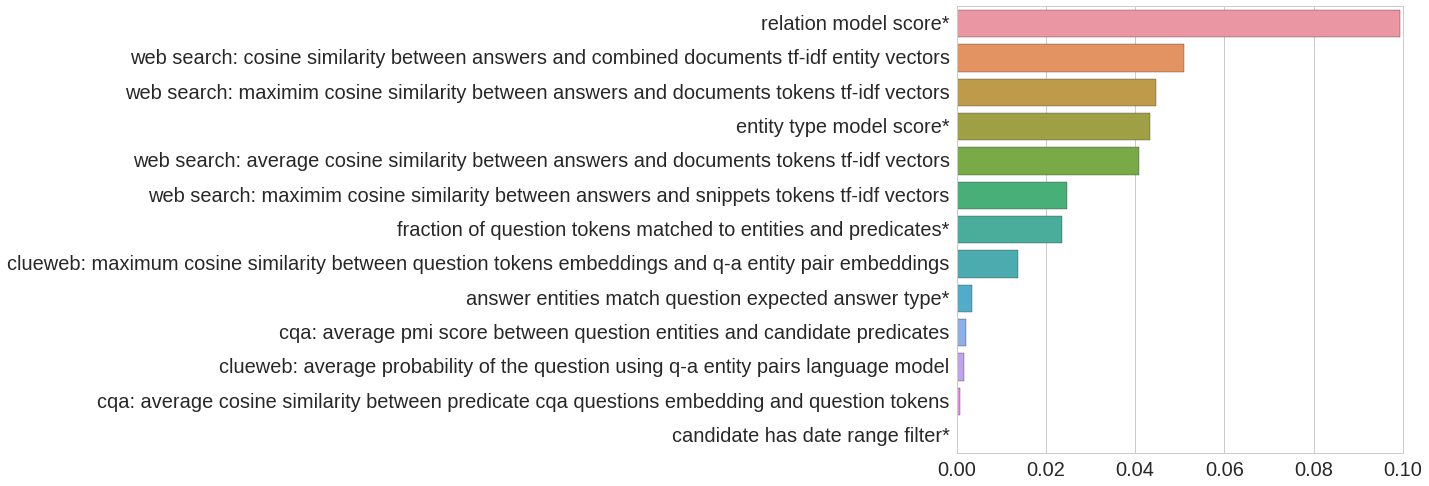
\includegraphics[width=0.9\textwidth]{img/feature_importances}
\caption{Importances of different text-based features for KBQA (features with * are not text-based and are provided for comparison)}
\label{fig:text2kb:feature_importances}
\end{figure}

The figure supports the observation that web search results features are the most useful, however, other text data sources also contribute to the improvement.

In summary, Text2KB significantly outperforms the baseline system, and each of the introduced components contributes to this improvement.
Web search results data turned out to be the most useful resource, and it significantly improves the quality by helping with question entity identification and candidate ranking.
Next, we analyze the system performance in more detail, and investigate factors for future extension.

\subsubsection{Analysis}
\label{subsubsec:text2kb:analysis}

We have shown that Text2KB outperforms the baseline.
We now investigate how our system would compare to other systems on the same benchmark; then, we investigate in depth the different error modes, which helps identify the areas of most substantial future improvements. 

% Don't have a better name for now. By generalization I mean whether our results are system specific or universally useful.
% \subsection{Generalization analysis}


\begin{table}
\centering
\caption{Average Recall (R), Precision (Pr), and F1 for Text2KB (our system), STAGG and their combinations}
\label{table:text2kb:combine_stagg}
\begin{tabular}{| p{4cm} | p{1cm} | p{1cm} | p{1cm} | }
\hline
System & R & P & F1 \\
\hline
%Aqqu (baseline) \cite{ACCU:2015} & 0.604 & 0.498 & 0.494\\
% DIDN'T HAVE TIME TO IMPLEMENT THIS.
% Text-only baseline & & & & \\
Our system: Text2KB & 0.6354 & 0.5059 & 0.5223 \\
STAGG \cite{yih:ACL:2015:STAGG} & 0.607 & 0.528 & 0.525\\
\hline
Text2KB + STAGG & 0.5976 & 0.5343 & 0.5320 \\
Text2KB + STAGG (oracle) & 0.7144 & 0.5904 & 0.6056 \\
\hline
\end{tabular}
\end{table}

We took an existing KBQA systems and demonstrated that by combining evidence from knowledge base and external text resources we can boost the performance.
A reasonable question is whether the same approach will be helpful to other systems, \eg the currently best system STAGG \cite{yih:ACL:2015:STAGG}.
The differences between our baseline system Aqqu and STAGG lie in the components, \ie entity linking algorithm, a set of query templates and ranking methods, therefore our approach is complementary and should be helpful.
To support this claim, we made an experiment to combine answers of STAGG and Text2KB.
One of the advantages of the former is its set of filters, that restricts list results to entities of certain type, gender, \etc
Therefore, we combined answers of STAGG and Text2KB using a simple heuristic: we chose to use the answer returned by STAGG if the number of answer entities is less than in the Text2KB answer, otherwise we use the answer of our approach.
Table \ref{table:text2kb:combine_stagg} gives the results of the experiment, and as we can see the combination achieves slightly better average F1 score.
Alternatively, we can look at the oracle combination of the systems, which always chooses an answer with higher F1.
This experiment shows that that systems don't make exactly the same mistakes and therefore can be combined.
As we can see such a combination results in a performance of 0.6056, which is much higher than either of the systems.

WebQuestions dataset is rather small as a result, answers to 112 of the test questions involve a predicate that weren't observed in the training set, which may be a problem for approaches that rely on a trained lexicon.
We evaluated both systems on these questions, and indeed the performance is very low, \ie the average F1 score of Text2KB is 0.1640 compared to 0.1199 for STAGG\footnote{Unfortunately, the number of questions is too low to show statistical significance (p-value=0.16)}.

\begin{figure}
\centering
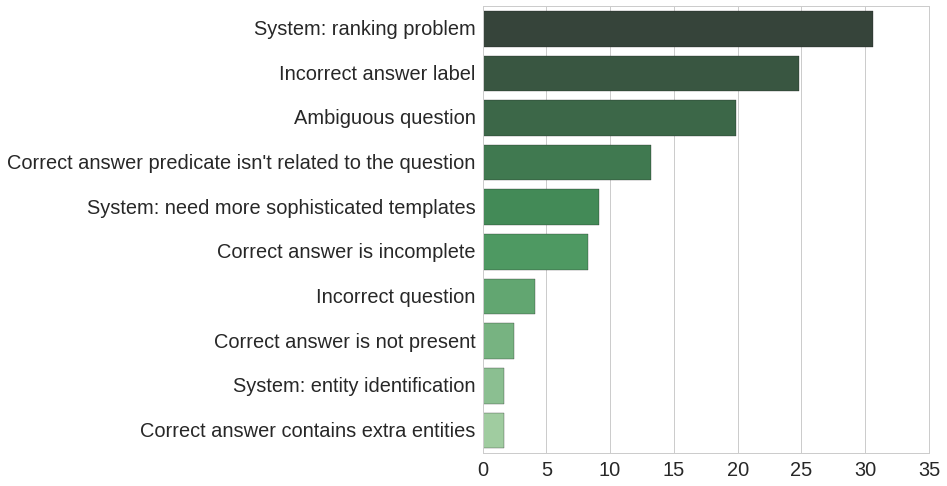
\includegraphics[width=0.45\textwidth]{img/error_analysis}
\caption{Distribution of problems with questions, where Text2KB returns an answer with F1$<$1}
\label{fig:text2kb:error_analysis}
\end{figure}

To get a better insights of the problems that remain, we collected 1219 questions for which Text2KB didn't return completely correct answer, \ie F1 score of the answer is less than 1.
We manually looked through a couple of hundreds of these examples and grouped the problems into several clusters.
The results are summarized on Figure \ref{fig:text2kb:error_analysis}.

As we can see candidate ranking is still the major problem, and it accounts for $~31\%$ of the cases.
The second most popular problem is incorrect ground truth labels (almost a quarter of errors).
For example: for the question \textit{when tupac was shot?''} the label says \texttt{Tupac 1994 assault} instead of \texttt{Las Vegas}.
Another set of questions have incomplete or overcomplete ground truth answer list.
Typical examples are questions asking for a list of movies, books, landmarks, \etc
The ground truth answer usually contains $\sim10$ entities, whereas the full list is often much larger.
This seems to be an artifact of the labeling process, where the answer was selected from the Freebase entity profile page.
The profile page shows only a sample of 10 entities from large lists and the others are hidden behind the ``NNN values total'' link.
About 20\% of the questions are ambiguous, \ie questions have no strict 1-1 correspondence with any of the predicates and can be answered by multiple without any obvious preferences.
% for the question \textit{``where is shakira from?''} the ground truth is the country - \texttt{Colombia}, while Text2KB returned her place of birth - \texttt{Barranquilla}.
For example, the question \textit{``what did hayes do?''} can be answered by profession, occupied position or some other achievements.
Another problem is when there is no predicate that answers the question.
For example, the question \textit{``what do people in france like to do for fun?''} doesn't have a good match among the facts stored in Freebase.
The ground truth entity \texttt{Cycling} comes from predicate related to the olympic sport competitions country participated in\footnote{\texttt{olympics.olympic\_participating\_country.athletes}}, which obviously isn't related to the question.
% In some cases there are entities that are very similar in meaning, but represented in Freebase by different ids and names.
% For example, the answer to the question \textit{``what is william taft famous for?''} is \textit{``President of the United States''}, which is a government position, but there is also a triple \texttt{[William Howard Taft, common.topic.notable\_for, US President]}, where the last entity represents a type of people who help the position, and is considered incorrect.

% This is nice, but probably is too little to mention.
% We also noticed, that in a small number of examples, the case of the correct answer entity and the answer returned by the system is different.
% For example, for the question \textit{``what fma stands for?''} the correct answer specified in the dataset is \textit{``FullMetal Alchemist''}, while the actual name of the entity is \textit{``Fullmetal Alchemist''}.
% The official evaluation script don't normalize the case and therefore considers this example incorrect.
% If we lowercase all entity names before comparison, the average F1 score of Text2KB becomes 0.5248.

As for the system errors, there are wins and loses introduced by each of our components.
Web search results helped identify the right question topical entity in a number of cases, \eg \textit{``what did romo do?''} mentions only the last name of the Dallas Cowboys quarterback and the baseline system were unable to map it to the right entity.
Web search results provides more than enough evidence that romo refers to \texttt{Tomo Romo}.
However, there are a number of loses, introduced by added unrelated entities.
For example, the entity \texttt{I Love Lucy} was added for the question \textit{``what was lucille ball?''}, because the term \textit{lucy} had high similarity with \textit{lucille}.
A portion of these problems can be fixed by a better entity linking strategy, \eg \cite{SMAPH_ERD:2014}.

% For the question \textit{``what did bruce jenner win gold medal for?''} the baseline system answered \textit{``1976 Summer Olympics''}, but web search results mention decathlon many times and thus Text2KB was able to rerank the candidates and return the entity \textit{``Athletics at the 1976 Summer Olympics - Men's Decathlon''}\footnote{Unfortunately, the entity selected as the answer during labeling is \textit{``Decathlon Challenge''}, which is a book Bruce Jenner wrote}.

An interesting example, when external text resources improved the performance is the question \textit{``what ship did darwin sail around the world?''}.
This is actually a hard question, because the ship entity is connected to the \texttt{Charles Darwin} entity through the ``knownFor'' predicate along with some other entities like \texttt{Natural selection}.
% \footnote{\texttt{user.lindenb.default\_domain.scientist.known\_for}
Thus, the predicate itself isn't related to the question, but nevertheless, the name of the ship \texttt{HMS Beagle} is mentioned multiple times in the web search results, and entity pair model computed from ClueWeb also has high scores for the terms ``ship'' and ``world''.

There are several major reasons for the loses, introduced by features based on external text resources.
Some entities often mentioned together and therefore one of them gets high values of cooccurrence features.
For example, the baseline system answered the question \textit{``when did tony romo got drafted?''} correctly, but since \texttt{Tony Romo} is often followed by \texttt{Dallas Cowboys}, Text2KB ranked the team name higher.
Another common problem with our features is an artifact of entity linking, which works better for names and often skips abstract entities, like professions.
For example, the correct answer to the question \textit{``what did jesse owens won?''} is an entity with the name \texttt{Associated Press Male Athlete of the Year}, which is rarely mentioned or it's hard to find such mentions.
Some problems were introduced by a combination of components.
For example, for \textit{``where buddha come from?''} a topical entity \texttt{Buddhism} was introduced from search results, and it generated \texttt{Gautama Buddha} as one of the answer candidates.
This answer was ranked the highest due to large number of mentions in the search results.
% In some cases search results aren't very relevant and only provide general information about question entity.

% Also problems of the original system persist, especially problems with the relation score model and popular predicates.

% I already mentioned this...
% WebQuestions dataset isn't free of noise and quite a few answers are actually incorrect for various reasons.
% When labeling the question ``what team does jordan own?'' mechanical turk workers had to select the answer from the page, corresponding to the country and not \textit{Michael Jordan} the basketball player.


% Non-relevant
% The first set of improvements come from the date range filter template, \eg for the question \textit{``who is the current leader of france 2010?''} our system returns a single correct result \textit{``Nicolas Sarkozy''} instead of the list of all French presidents.
% The type model score feature helped in some cases, where there is a clear indication of the type of entity, expected as the answer, \eg \textit{``which state did anne hutchinson found?''} - \textit{``Rhode Island''}.

In summary, we show that ideas behind Text2KB could be integrated into other systems and improve their performance.
The error analysis suggested that even though a significant number of questions in the WebQuestions dataset have incorrect or ambiguous ground truth labels, there is still a room for improvement.
In particular, the future work for Text2KB will include a better strategy for entity linking using external data sources and a better context model for entity mentions in text documents, which can put more weight on entities mentioned in the context related to the question.

\subsubsection{Conclusion}
\label{subsubsec:text2kb:conclusion}

Our work showed that unstructured text resources can be effectively utilized for knowledge base question answering to improve query understanding,  candidate answer generation and ranking.
We focused on three particular techniques and associated text information sources: web search results for query understanding and candidate ranking, community question answering data for candidate generation, and text fragments around entity pair mentions for ranking. Certainly, there are more resources that could be potential adapted, \eg entity profile pages like Wikipedia, news sources, textbooks, and many others. However, we believe that the proposed approach is general enough that it could be extended and successfully incorporate these other diverse text sources.

In the future, we plan to extend our work to the more open setup, similar to the QALD hybrid task, where questions no longer have to be answered exclusively from the KB. This would require extending the described techniques, and creating new QA benchmarks.

% =-=-=-=-=-=-=-=-=-=-=-=-=-=-=-=-=-=-=-=-=-=-=-=-=-=-=-=-=-=-=-=-=-=-=-=-=-

\subsection{Hybrid Question Answering over Knowledge Bases and Semantically Annotated Text Collections}
\label{subsec:text+kb}

Experiments of the previous chapter demonstrated that external text data can be useful for knowledge base question answering systems.
However, such an approach can only help with the problem of lexical gap, \ie mapping from natural language phrases to knowledge base concepts.
It doesn't deal with the problem of KB incompleteness, \ie in Text2KB system text resources cannot compliment the knowledge from the database, it only extends its representation.

\begin{figure}
\centering
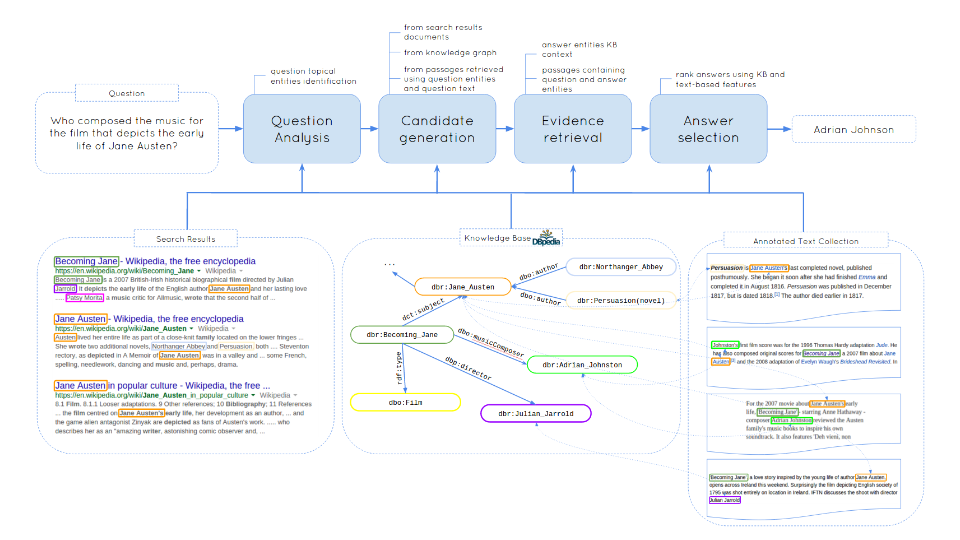
\includegraphics[width=\textwidth]{img/text_and_kb}
\caption{Architecture of a hybrid factoid question answering system, that uses a combination of structured knowledge base and unstructured text data}
\label{fig:text_kb}
\end{figure}

In this section I propose a novel hybrid QA architecture, that combines unstructured text and structured knowledge base data for joint inference.
Figure \ref{fig:text_kb} gives a general overview of the proposed system.
The idea is to extend the documents representation with annotations of KB entity mentions, which essentially creates additional edges in the knowledge graph.
These edges connecting KB entities with text fragments can be traversed by a QA system in both directions in order to get more syntactic (from entity to text) or semantic (from text to entity) information.
In addition, text fragments, that mention 2 different entities close to each other can serve as an addition knowledge triple.
Unlike information extraction approaches, however, we don't try to extract the predicate and get rid of all the other information stated in a sentence.
In the proposed approach we are going to use text similarity metrics to retrieve such triples.

The main stages of the QA pipeline are the following:
\begin{itemize}
\setlength\itemsep{0em}
\item \textbf{Pre-processing}: identify mentions of KB entities in text document collection and index the documents text and mentions in separate fields
\item \textbf{Topical entity identification}: search the text collection using question (or reformulated question \cite{AgichteinLG01}) as a query and use an approach similar to \cite{cornolti2014smaph} to detect question topical entities
\item \textbf{Candidate generation from text}: extract candidate answer (or intermediate answer) entities with evidence from the retrieved text documents using existing techniques, e.g. \cite{tsai2015web}.
\item \textbf{Candidate generation from KB}: explore the KB neighborhood of question topical entities and entities extracted from text documents on the previous step
\item \textbf{Candidate generation from KB \& Text}: use entity and text index to find entities mentioned near question topical entity and question terms in the document collection
\item \textbf{KB evidence extraction}: match neighborhood of answer entities (entity type and other entities) against the question to get additional evidence
\item \textbf{Text evidence extraction}: estimate the similarity between the collection text fragments mentioning question and answer entities and the question text
\item \textbf{Rank candidate}: rank candidate answers using evidence extracted from the KB as well as from text
\end{itemize}

As a motivating example, let's consider the following question from the QALD dataset: ``\textit{Who composed the music for the film that depicted the early life of Jane Austen?}''.
Even though it's quite easy to identify the ``\texttt{Jane Austen}'' entity in the question, the knowledge base (dbPedia in this example) cannot help us to determine which movie is being referred to.
However, there are plentiful of documents on the web, that describe the plot of the \texttt{Becoming Jane} movie, and a system can use the proximity of terms from the question \textit{``... depicted early life of Jane Austen''} to the movie entity.
Unfortunately, extracting the name of the composer from these documents is quite challenging, but this task can be easily accomplished by checking the value of the \texttt{musicComposer} property in the knowledge base.
At the end, for each candidate answer entity, we have all the KB information and passages that mention this entity as evidence to help with the correct answer selection.


\subsubsection{Evaluation}
\label{sec:factoid_evaluation}

To evaluate the performance of the proposed approach I will compare it against several alternatives on multiple datasets.
The baselines I will compare against include a semantically enriched text-based system QuASE \cite{Sun:2015:ODQ:2736277.2741651}, a hybrid YodaQA system, designed to be an open source analogue to IBM Watson \cite{baudivs2015yodaqa} and open question answering approach of \cite{Fader:2014:OQA:2623330.2623677}.

Most of the works in question answering have been evaluated on the TREC QA datasets.
These datasets come with a set of regular expression patterns that can judge an answer as correct or incorrect.
Unfortunately, these patterns aren't complete and researchers often end up re-validating the answers of their systems manually \cite{Sun:2015:ODQ:2736277.2741651,tsai2015web}.
Unlike most of the previous approaches, however, the proposed system aims at retrieving KB entities as answers of the questions.
Therefore, I'm planning to annotate TREC QA datasets answers with KB entity identifiers.
The proposed system can use the web as the corpus and query it using Bing Search API\footnote{https://datamarket.azure.com/dataset/bing/searchweb}.
dbPedia, Freebase and Reverb extractions \cite{FaderSE11} are examples of schema-based and open knowledge bases that can be used for the experiments.
The metrics used for evaluation typically include accuracy and mean reciprocal rank (MRR).

Most of the recent work on knowledge base question answering and semantic parsing have been evaluated on the WebQuestions dataset \cite{BerantCFL13:sempre}.
I will compare the proposed approach with previous results \footnote{http://goo.gl/sePBja} on this dataset.
Again, web can be used as a text collection which can be queried using Bing Search API.
% Relation extraction patterns can be mined using distant supervision from ClueWeb collection using publicly available dataset of Freebase annotations \cite{gabrilovich2013facc1}.

\textbf{New factoid question answering dataset}.
WebQuestions dataset has certain limitations.
Most of the questions mined using Google Suggest API have very similar structure and lexicon, which makes it easier for systems to learn a mapping from natural language phrases to KB predicates.
Furthermore, answers to the question were labeled using entities' Freebase profile pages, which only displays relations in the close proximity to the target entity.
This makes it possible to exploit a small set of templates to generate candidate answer queries.
To overcome this limitations I'm designing a new factoid QA dataset, derived from questions posted to Yahoo! Answers CQA website.
A set of heuristics can be used to filter factoid questions from more general opinion, recommendation, \etc questions.
For example, we can select a subset of QnA pairs with at least one entity in the question and answer, without personal pronouns, words like ``\textit{recommend}'', ``\textit{suggest}'', superlative adjectives like ``\textit{best}'', \etc.
Next this QnA pairs will be further labeled by Mechanical Turk users, who will determine if the questions are indeed factoid and non-subjective and select the actual answer entity from the list of entities, mentioned in the answer text.
The preliminary analysis showed, that from 3.8M QnA pairs from Yahoo! Answers WebScope collection, 80K passed the heuristics filters described above and about 30\% of them are actually good factoid questions.
Examples of questions are: ``\textit{What was James Bond's wife's name?}'', ``\textit{What is the name of the second US astronaut to land on the moon?}'', ``\textit{When was the first "cartoon human" movie?}'', ``\textit{What movie did Joe Pesci describe kids as "YUTS"?}''.
I expect this dataset to contain ~10K real user questions annotated with answer entities, which can be used for future research in question answering in both knowledge base and general factoid question answering.

\section{Summary}
In this section we considered two different ways of combining unstructured and structured data to improve factoid question answering.
Relation extraction from question-answer pairs aims at filling some gaps in KB fact coverage, whereas semantic annotations of text documents provides a way to incorporate information available in unstructured text documents for reasoning along with KB data to improve the performance of factoid question answering.

Factoid questions represent just a part of user information needs. Many problems require more elaborate response, such as a sentence, list of instructions or in general a passage of text.
Such questions are usually referred to as non-factoid questions and they will be the focus of the next Chapter.

\clearpage

%--- THE NEXT PIECE IS OLDER, NEED TO REVIEW

%Question answering from text corpora typically starts by retrieving a set of potentially relevant documents using the question (or some transformation of the question \cite{AgichteinLG01}) as the query, and then extracting entities, phrases, sentences or paragraphs believed to be the answer to the question.
%However, the information available in the retrieved pieces of text is very limited and often not enough to decide whether it can be the answer to the given question.
%For example, below is one of the questions from TREC QA 2007 dataset:\\
%\textit{``What republican senators supported the nomination of Harriet Miers to the Supreme Court?''}\\
%A candidate answer sentence \textit{``Minority Leader Harry Reid had already offered his open support for Miers.''} mentions a senator ``Harry Reid'' and clearly says about his support of the nomination.
%However, ``Harry Reid'' is not a correct answer to the question because he is a member of the Democratic party.
%This information is not available in the answer candidate sentence, but it is present as one of the properties in Freebase: [Harry Reid, political\_party, Democratic party]\footnote{Actually, in Freebase the entities are connected by a path of length 2 through a mediator node. The predicates on the path are: /government/politician/party and /government/political\_party\_tenure/party}.
%Therefore, by looking into the knowledge available about the mentioned entities a QA system can make a better judgment about the candidate answer.

% THIS IS THE CORRESPONDING PIECE ON KBQA, I DON'T REALLY LIKE IT

% Question answering over linked data (knowledge bases) converts a natural language question into a structured query, such as SPARQL.
%The main challenge for such systems is to map words and phrases from the question to the corresponding entities and predicates from a KB.
%Usually, such lexicon is built during training using ground truth question-query pairs \cite{CaiY13} or question-answer pairs \cite{BerantCFL13:sempre}.
%Improvements were made by extending the lexicon using Wikipedia and patterns expressing certain predicates obtained via distant supervision \cite{bastmore:cikm:2015:aquu,BordesCW14:emnlp,ReddyLS14,yih:ACL:2015:STAGG,YaoD14}.
%But still, the amount of available labeled or weakly labeled training data is much smaller than the amount of unstructured data.
%This unstructured data will complement the learned lexicon, e.g. even if a question about a certain predicate wasn't seen during training, a set of text paragraphs mentioning both of the related entities can provide a QA system with enough evidence to make the correct decision.

% chap4.tex
%

\mychapter{Non-factoid Question Answering}

Most of the questions that people have are not factoid and cannot be simply answered with a name, date or a number.
Typically, such questions require a more elaborate fragment of text as an answer.
Traditionally, question answering systems turn to web documents that might contain some relevant passages to be used as an answer.

\noindent
In this chapter, I summarize the proposed work for improving automatic non-factoid question answering by better understanding the structure of web documents and relationships between their parts and fragments.
% In particular, we first focus on ...., and then try to ...
% The goal is 

\section{Utilizing the Structure of Web Pages}

Non-factoid questions are typically answered with a relatively long paragraph of text\footnote{TREC LiveQA'15 challenge limits the answer to 1000 characters}.
This fact and the nature of questions limits the utility of structured KB resources.
One of the main challenges for non-factoid question answering is matching between the question needs and the information expressed in text fragment.
Analysis of TREC LiveQA 2015 participants \cite{savenkov2015liveqa} revealed that the quality of answers extracted from previously posted similar questions is typically higher than from regular web passages.
Therefore, non-factoid QA system would benefit from the information on which questions does a paragraph of text answer.
This information can often be extracted from the structure of a web document, e.g. forum threads, FAQ pages or various CQA websites.
Alternatively, we can train a model to predict whether a paragraph answers a given question using titles, subtitles and surrounding text of a web page.

\begin{figure}[h]
\centering
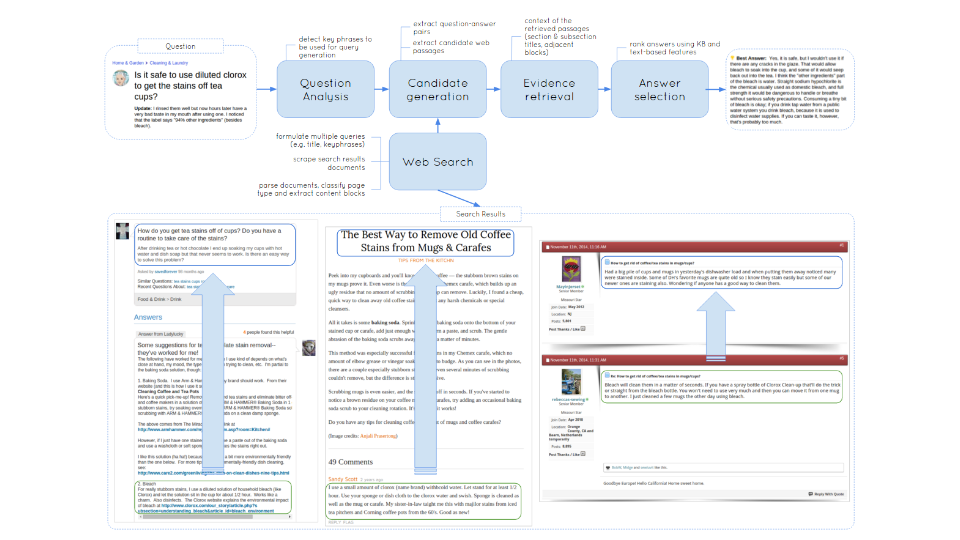
\includegraphics[width=\textwidth]{img/web_page_structure_nonfactoid}
\label{fig:web_page_structure_nonfactoid}
\caption{Using web page structure information for non-factoid question answering}
\end{figure}

My proposal for non-factoid question answering can be summarized as follows:
\begin{itemize}
\setlength\itemsep{0em}
\item \textbf{CQA candidate generation}: retrieve a set of question-answer pairs by searching a CQA archive\footnote{https://answers.yahoo.com/}
\item \textbf{Web document retrieval}: retrieve a set of documents by querying web search with the question (and queries generated from it)
\item \textbf{Web candidate answer generation}: classify web page into one of the following types: article, forum thread, FAQ page, CQA page, other. Extract key elements using type-specific extractors (QnA pairs, FAQ and CQA pages, forum question and posts and article passages with the corresponding titles, subtitles and surrounding text).
\item \textbf{Ranking}: Rank the generated candidate answers by building on techniques from existing research \cite{surdeanu2011learning}.
\end{itemize}


\section{Evaluation}
LiveQA


\section{Summary}

% chap5.tex
%

\mychapter{Human Interaction with Question Answering Systems}
\label{chapter:users}

\noindent

Modern automatic question answering systems are still far from AI machines, that we often imagine or see in the movies.
Many user information needs are still unanswered by existing techniques.
For example, only 36\% of answers of a winning approach from TREC LiveQA 2015 shared task were judged good or excellent.
And it's unlike to become 100\% as users are not perfect either and often the questions they ask are hard to understand or ambiguous.
Therefore, it is important to improve not only the answering aspect of the systems, but also interaction experience altogether.
In this chapter I propose a couple of research directions in this area, which can help improve the overall success rate by engaging in a dialog with the user.
More specifically, in Section \ref{sec:user:hints} I describe strategic search hints for complex informational tasks, which a system can show to the user in case its response was not satisfactory.
We discuss the effects such hints have on the user success rate and satisfaction.
However, this type of intervention leaves all the heavy lifting of formulating good search queries on the user.
Section \ref{sec:user:clarification} discuss how a system can engage in a dialog by asking some clarification questions to resolve ambiguities in user's question.

%-=-=-=-=-=-=-=-=-=-=-=-=-=-=-=-=-=-=-=-=-=-=-=-=-=-=-=-=-=-=-=-=-=-=-=-
\section{Search Hints for Complex Informational Tasks}
\label{sec:user:hints}

Search engines are ubiquitous, and millions of people of varying experience use them on daily basis.
Unfortunately, not all searches are successful.
Bilal and Kirby \cite{Bilal:2002:DSI:637512.637516} reported that about half of the participants of their user study felt frustration when searching.
Xie and Cool \cite{xie2009understanding} demonstrated that most of the time users have problems with formulating and refining search queries.
Besides good retrieval performance, a successful search requires users to possess certain skills.
Search skills can be trained, e.g. Google offers a course\footnote{http://www.powersearchingwithgoogle.com} on improving search efficiency.
Although very useful, such courses are time consuming and detached from real search problems of these particular users.
Displaying search hints is another technique that has both learning effect, and offers immediate assistance to the user in solving her current search task.
Moraveji et al. \cite{Moraveji:2011:MIU:2009916.2009966} demonstrated that hints, suggesting certain search engine functionality, help people find answers more quickly, and the effect is retained after a week without hints.

% Besides the awareness about search tools available, adopting general search strategies is extremely important when dealing with a difficult search task.
In my thesis I propose to explore {\em strategic} search hints, that are designed to guide a user in solving her search problem.
More specifically, we chose the divide-and-conquer strategy, \ie splitting an original difficult question into smaller problems, searching answers to the subtasks and combining them together.
Two sets of strategic hints were manually designed: {\em generic} hints describing the divide-and-conquer strategy in general and {\em task-specific} hints providing a concrete strategy to solve the current search task.
To evaluate the effect of the hints on behavior and search success we conducted a user study with 90 participants.
The results of the user study demonstrate that well-designed task-specific hints can improve search success rate.
In contrast, generic search hints, which were too general and harder to follow, had negative effect on user performance and satisfaction.

\subsection{User Study}

\begin{figure}
\centering
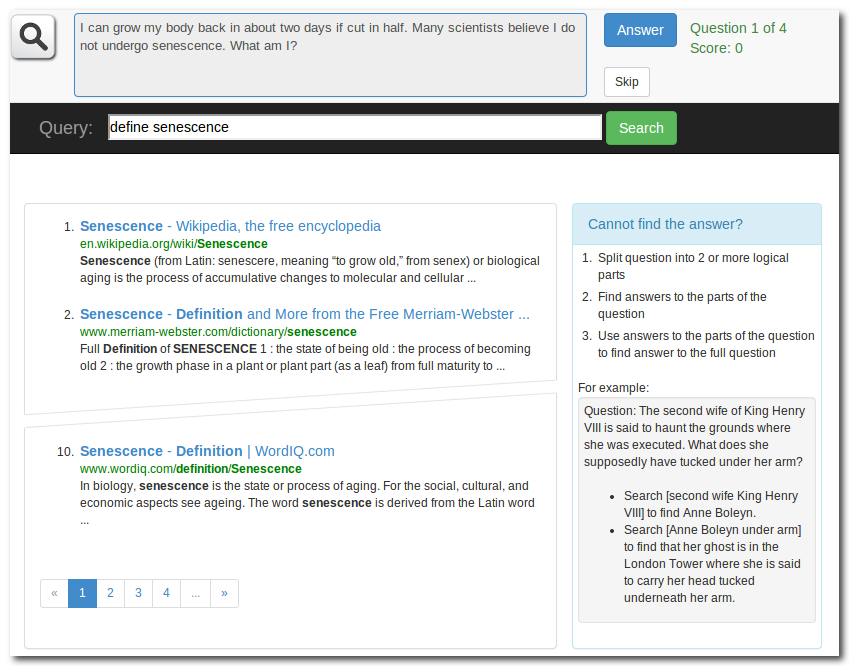
\includegraphics[width=0.75\textwidth]{img/ufindit}
\caption{The interface of the search game used in the study}
\label{figure:ufindit}
\end{figure}

To estimate the effect of strategic search hints on user behavior we conducted a study in a form of a web search game similar to ``a Google a Day''\footnote{http://www.agoogleaday.com/} and uFindIt \cite{Ageev:2011:FYG:2009916.2009965}. Participants were hired using Amazon Mechanical Turk\footnote{http://www.mturk.com/}. 

The goal of the web search game used in the user study is to find answers to several questions with the provided web search interface (Figure \ref{figure:ufindit}). 
Players are instructed not to use any external tools.
% Figure \ref{figure:ufindit} shows the interface of the game.
The questions are given one by one and since tasks might be too difficult, a chance to skip a question was provided, although users were instructed that effort put into solving a question will be evaluated.
To answer a question each player needs to provide a link to a page containing the answer as well as its text.
The answer is automatically verified and a popup box notifies a player if the answer is incorrect (since the answer can be formulated differently, presence of a keyword was checked).
A player can then continue searching or skip the question when she gives up.
A bonus payment was made to players who answer all questions correctly.
We used Bing Search API\footnote{http://www.bing.com/toolbox/bingsearchapi} as a back-end of the game search interface.
All search results and clicked documents were cached so users asking the same query or clicking the same page got the same results.
At the end of the game a questionnaire was presented asking for feedback on user satisfaction with the game, prior experience and other comments.

\begin{table}[tbh]
\centering
\caption{Search tasks used for the study, and specific search hints shown to one of the user groups}
\label{table:tasks}
\begin{tabular}{|p{1cm}|p{4.5cm}|p{4.2cm}|p{6.0cm}|} \hline
 & Question & Correct Answer & Specific hints \\ \hline
Task 1 & I can grow body back in about two days if cut in half. Many scientists think I don't undergo senescence. What am I? & Senescence means ``biological aging''. Hydra is considered biologically immortal and regenerates fast. & \parbox[t]{6cm}{
1. Find what is senescence\\
2. Find who does not undergo senescence\\
3. Find who can also regenerate body and choose the one that satisfies both conditions} \\ \hline
Task 2 & Of the Romans "group of three" gods in the Archaic Triad, which one did not have a Greek counterpart? & Archaic Triad includes Jupiter, Mars and Quirinus. Among those Quirinus didn't have a Greek counterpart. &
\parbox[t]{6cm}{
1. Find the names of the gods from the Archaic triad\\
2. For each of the gods find a Greek counterpart
}\\ \hline
Task 3 & As George surveyed the ``waterless place'', he unearthed some very important eggs of what animal? & "Gobi" in Mongolian means ``Waterless place''. The first whole dinosaur eggs were discovered there in 1923. & \parbox[t]{6cm}{
1. Find what is the ``waterless place'' mentioned in the question?\\
2. Search for important eggs discovery in this ``waterless place''}\\ \hline
Task 4 & If you were in the basin of the Somme River at summers end in 1918, what language would you have had to speak to understand coded British communications? & Cherokee served as code talkers in the Second Battle of the Somme. & \parbox[t]{6cm}{
1. Find the name of the battle mentioned in the questions\\
2. Search for which coded communications language was used in this battle\\
} \\ \hline
\end{tabular}
\end{table}

The tasks for the study were borrowed from the ``A Google a Day'' questions archive.
Such questions are factual, not ambiguous and usually hard to find the answer with a single query, which makes them interesting for user assistance research.
We filtered search results to exclude all pages that discuss solutions to ``A Google a Day'' puzzles.
To do this we removed pages that mention a major part of the search question or ``a google a day'' phrase.
To keep users focused throughout the whole game we limited the number of questions to 4.
The tasks are described in Table \ref{table:tasks} and were presented to all participants in the same order to ensure comparable learning effects.

The questions have multiple parts and to solve them it is helpful to search for answers to parts of the questions and then combine them.
In one of the previous studies we observed, that most of the users didn't adopt the divide-and-conquer strategy, but kept trying to find the ``right'' query.
We decided to estimate the effect of strategic search hints, suggesting users to adopt the new strategy.

We built 2 sets of strategic hints: \textit{task specific} and \textit{generic}.
Task-specific hints described steps of one of the possible solutions to each question (Table \ref{table:tasks}).
Second set contained a single hint, which was shown for all tasks. Generic hint described the divide-and-conquer strategy:\\
\hrule
\begin{enumerate} \itemsep0pt \parskip0pt \parsep0pt
\item Split the question into 2 or more logical parts
\item Find answers to the parts of the question
\item Use answers to the parts of the question to find answer to the full question
\end{enumerate}

For example, the question: ``The second wife of King Henry VIII is said to haunt the grounds where she was executed. What does she supposedly have tucked under her arm?''
\begin{enumerate} \itemsep0pt \parskip0pt \parsep0pt
\item Search [second wife King Henry VIII] to find Anne Boleyn.
\item Search [Anne Boleyn under arm] to find that her ghost is in the London Tower where she is said to carry her head tucked underneath her arm.
\end{enumerate}
\hrule

To control for the learning effect demonstrated in \cite{Moraveji:2011:MIU:2009916.2009966}, each user was assigned to one of the three groups:
\begin{enumerate}\itemsep0pt \parskip0pt \parsep0pt
\item users who didn't get any hints
\item users who got task-specific hints
\item users who got the generic hints
\end{enumerate}


\subsection{Results}

From 199 unique participants, who clicked the HIT on Amazon Mechanical Turk only 90 players finished the game.
We further examined all games manually and filtered out 9 submissions for one of the following reasons: lack of effort (e.g. skipped several tasks after none or a single query) or usage of external resources (e.g. the answer was obtained without submitting any queries or results explored didn't contain the answer).
Furthermore, 10 players from the group which received hints indicated in the survey that they didn't see them, so we filtered out those submissions and finally we had 71 completed games (29 for no hints, 20 for task-specific hints and 22 for generic hints groups).

\subsubsection{Effects of Search Tips on Performance}

In order to measure search success rate we looked at the number of questions answered correctly by different groups of users\footnote{Since users were allowed to skip a question we are counting the number of questions that were eventually solved correctly even if a player made some incorrect attempts}.
Figure \ref{figure:hints:task_success} shows that success rate is higher for users who saw task-specific hints compared to users who didn't get such assistance.
Surprisingly, having the generic hint decreased the success rate, although users could easily ignore a hint they didn't like.
A possible explanation is: generic hints were harder to follow and users who tried and failed became frustrated and didn't restart their searches.

% Similar to \cite{Moraveji:2011:MIU:2009916.2009966} we looked at the average time to answer a question (for this analysis we removed games where a user didn't find the answer and skipped the task).

The plot of average time to answer a question on Figure \ref{figure:hints:task_time} doesn't show an improvement for the task-specific hints group, except for the question 1.
Our task-specific hints represent a possible way to solve a problem and there is no guarantee, that it is the fastest one.
It is worth noting, that users from the generic search hint group had slightly higher variance in success time, which can probably be explained by the fact that some users were successful in finding the right way to follow the hint and some other users struggled with it much longer.
Another insight comes from the number of incorrect attempts users made.
Figure \ref{figure:hints:incorrect} demonstrates the average number of incorrect answer attempts for all groups of users.
Although the variance is high, there is a tendency for users who saw task-specific hints to make less attempts than both other groups.
This is not in direct correspondence with time spent on the game.
It seems that the users who saw a clear strategy to solve the question were less likely to notice plausible, but incorrect solution.
Moreover, we analyzed texts of incorrect answers, and can conclude that a big part of incorrect submission are due to users trying all possible options they found on the way, even if these options are clearly wrong.
% We should note, that unfortunately we didn't limit the number of attempts per problem, thus strategy to verify an answer by submitting it made sense.

\begin{figure}[h]
\centering
  \begin{subfigure}{0.32\textwidth}
  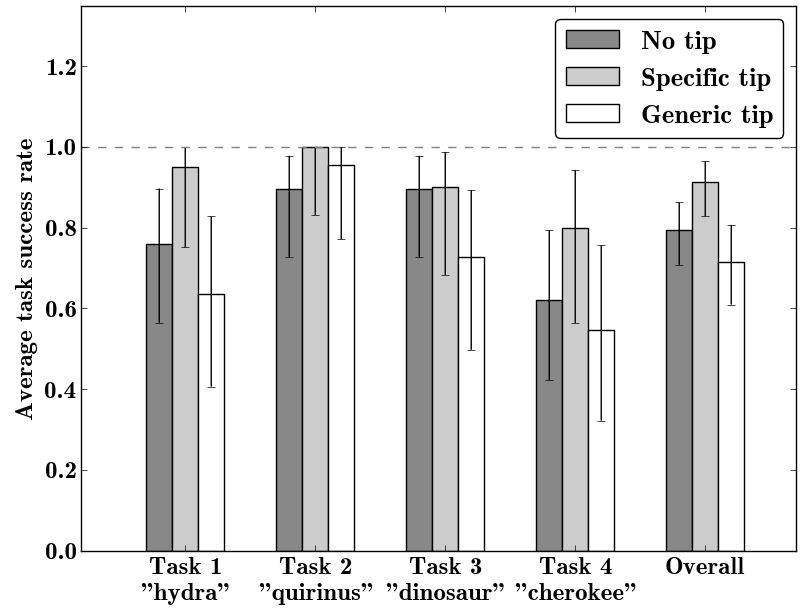
\includegraphics[width=\textwidth]{img/success_per_task}
  \caption{Success rate per task for each group of participants}
  \label{figure:hints:task_success}
  \end{subfigure}
  \begin{subfigure}{0.32\textwidth}
  \centering
  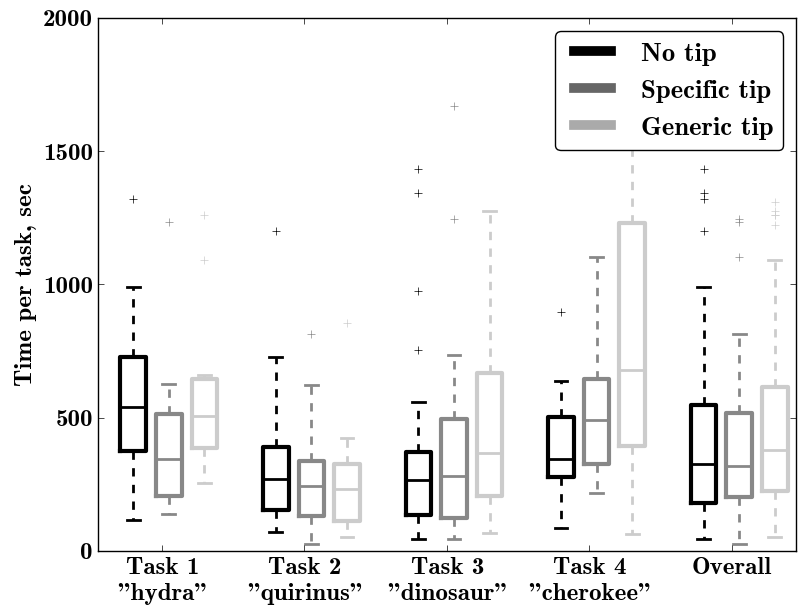
\includegraphics[width=\textwidth]{img/time_per_task}
  \caption{Task completion time for each group of players}
  \label{figure:hints:task_time}
  \end{subfigure}
  \begin{subfigure}{0.32\textwidth}
  \centering
  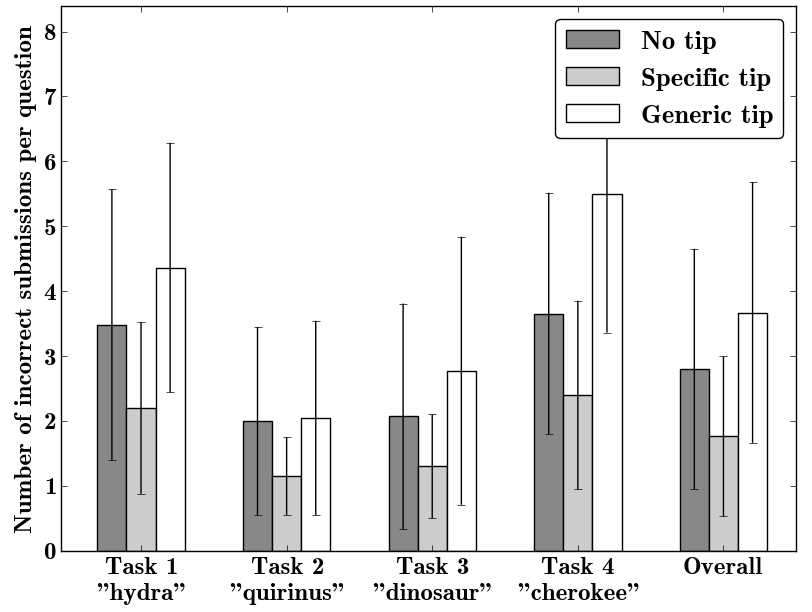
\includegraphics[width=\textwidth]{img/incorrect}
  \caption{The number of incorrect submission attempts per question for all groups of users}
  \label{figure:hints:incorrect}
  \end{subfigure}
\caption{Results of the user study on the effectiveness of strategic search tips on search task success rate}
\label{fig:hints:results}
\end{figure}

\begin{figure}[h]
\centering
\begin{subfigure}[t]{0.32\textwidth}
	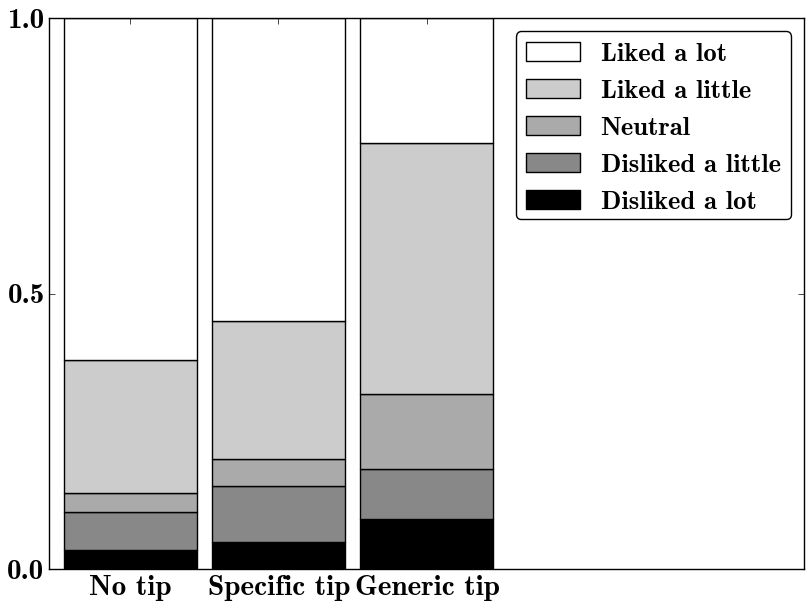
\includegraphics[scale=0.26]{img/liked}
	\caption{How did you like the game?}
    \label{figure:survey:liked}
\end{subfigure}
\begin{subfigure}[t]{0.32\textwidth}
	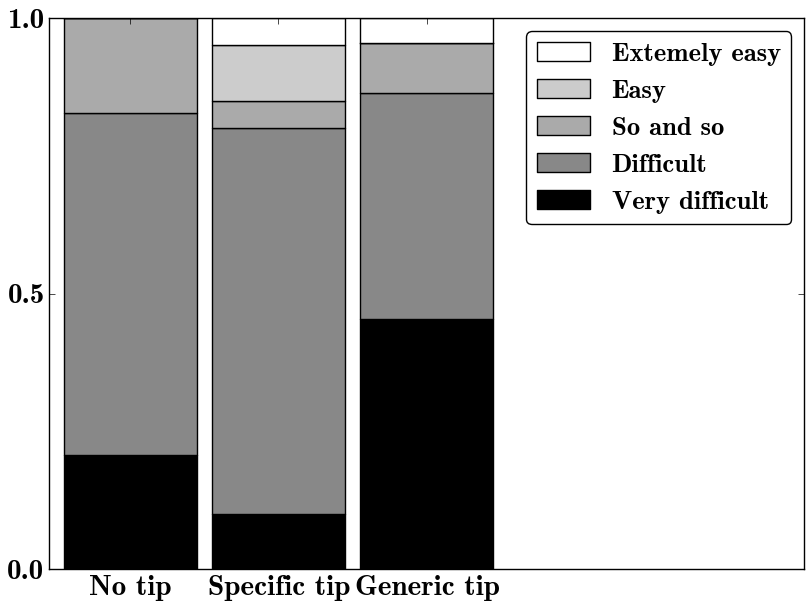
\includegraphics[scale=0.26]{img/difficult}
	\caption{How difficult was the game?}
    \label{figure:survey:difficult}
\end{subfigure}
\begin{subfigure}[t]{0.32\textwidth}
	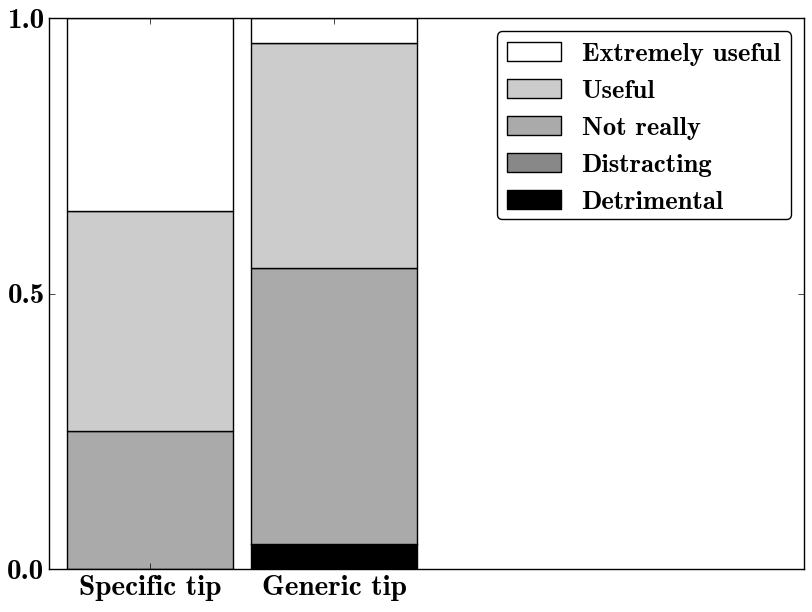
\includegraphics[scale=0.26]{img/useful}
	\caption{Were search hints useful to you?}
    \label{figure:survey:useful}
\end{subfigure}
\caption{Proportions of replies to some of the survey question for each group of users}
\label{figure:hints:survey}
\end{figure}

We also looked at other search behavior characteristics: number of queries submitted, number of clicks made, average length of the queries. The variance in these characteristics was too high to make any speculations regarding their meaning.

\subsubsection{Effects of Search Tips on User Experience}

Finally, we looked at the surveys filled out by each group of users.
Figure \ref{figure:hints:survey} presents proportions of different answers to three of the questions: ``How did you like the game?'', ``How difficult was the game?'' and ``Were search hints useful to you?''.
Surprisingly, user satisfaction with the game was lower for users who saw hints during the game and users who didn't get any assistance enjoyed it more.
The replies to the question about game difficulty are in agreement with the success rate: users who saw task-specific hints rated difficulty lower than participants who struggled to find the correct answers.
The game was very difficult on average, however, some participants from the group who received task-specific hints surprisingly rated it as very easy, which suggests that our hints do help users.
This is supported by the answers to the last question on whether hints were helpful (Figure \ref{figure:survey:useful}).

To summarize, the results of the conducted user study suggest that specific search hints can be helpful, which is indicated by higher success rate, lower number of incorrect attempts and positive feedback in the end of study survey.
In contrast, generic hints can have negative effect on user experience, which is indicated by lower success rate, increased number of incorrect attempts and higher perceived tasks complexity according to the survey.

\subsection{Summary}
In this section we studied the effect of strategic search hints on user behavior. 
The conducted user study in a form of a web search game demonstrated the potential of good hints in improving search success rate.
However, to be useful, they should be designed carefully.
Search hints that are too general can be detrimental to search success.
We also find that even searchers who are more effective using specific search hints, feel subjectively less satisfied and engaged than the control group, indicating that search assistance has to be specific and timely if it is to improve the searcher experience.

We should note, that specific search hints used in this work were manually generated and an interesting question of future work is how to generate such useful hints automatically.
It should be possible to learn strategies applied by the experienced search users and suggest them to the rest.

%-=-=-=-=-=-=-=-=-=-=-=-=-=-=-=-=-=-=-=-=-=-=-=-=-=-=-=-=-=-=-=-=-=-=-=-
\section{Clarification Questions}
\label{sec:user:clarification}

Nowadays, with intelligent assistants and chat bots we are observing a shift towards natural language interfaces, which will enable richer interaction between a human and computer, in particular question answering.
Most of the existing systems are one-sided, \ie they operate by returning an answer in a response to a user question.
A richer model will inevitably lead to a dialogue rather than request-response kind of communication.
There are many practical aspects of maintaining a dialogue for question-answering.
For example, many questions that user ask are not clear or ambiguous, \eg ``How can I bring up my pictures that I had in windows 8.1?''.
Instead of returning a useless answer, a system can detect a problem with the question and come back with a clarification question to the user, which would allow to use the response to generate a better answer.

The research I propose towards a dialog-based QA are:
\begin{itemize}
\item Study user behavior patterns associated with asking clarification questions
\item Build a classification model to predict when a question requires a clarification
\item Choose a subset of clarification types and design a system to generate questions in response to ambiguous user queries.
\end{itemize}

For our behavior study we are planning to use data from StackExchange CQA website\footnote{http://stackexchange.com/}, which allows users not only answer the posted questions, but also comment on them and many comments are indeed clarification questions (Figure \ref{figure:user:clarification:stackexchange}).
We will filter out questions, that contain a question comment and perform an exploratory study of different types of forms of these responses.

Preliminary analysis suggested, that there are many different kinds and nature of clarifications.
Some address the general quality of user's question, \eg ``Is this a duplicate of [...]''.
Another fraction of the clarifications address certain ambiguities present in the question or in the described situation, \eg ``In what way is it oversize -- too high, wide, or both? What are the dimensions?''.
These types of clarifications doesn't usually refer to any particular answer or solution.
Finally, some comments are actually proposing certain answers, which might be trivial (``Have you tried contacting the company's customer support?'') or might not work (``Have you tried adjusting the fill valve / float arm so the tank fills higher?'').

\begin{figure}[h]
\centering
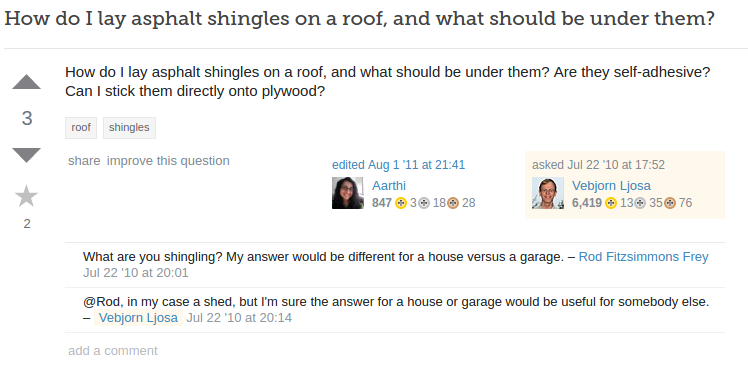
\includegraphics[width=0.7\textwidth]{img/stackexchange_example}
\caption{A question and clarification comment posted by users on StackExchange question answering website}
\label{figure:user:clarification:stackexchange}
\end{figure}


In my thesis I'm planning to focus on a subset of questions, that are ambiguous and therefore cannot be reliably answered without a clarification.
We will select a subset of such questions from the dataset, and train a machine learning model to predict whether a question requires a clarification or can be answered as is.
This problem is somewhat similar to the question answerability, studied in \cite{dror2013will,shah2010evaluating}.
However, the problem here is more specific, as we can imagine that an ambiguous question can still receive an answer, and questions that are not ambiguous can be left unanswered, for example if the community did not know the answer.
However, the features explored in these works will probably be useful in our scenario as well.
For evaluation, I will split the original dataset into training and test sets and use precision and recall classification metrics.

Finally, the next stage after we detected an ambiguous question is to automatically ask a clarification question.
I'm planning to explore two possible approaches: template-based and recurrent neural networks based approaches.
Template-based approach will target a subset of potential questions, \eg ``What type of <OBJ> do you have?'', ``How old is your <OBJ>?'', \etc.
Such templates can be automatically mined from the collection, and the only problem for the model is to detect the object to ask about, which can be solved by training another machine learning model.

Recurrent neural networks showed impressive results in multiple areas, such as machine translation \cite{sutskever2014sequence}, image caption generation \cite{vinyals2015show} and dialogs \cite{vinyals2015neural}.
The later work is especially relevant and for this experiment I'm planning to build on it use a bidirectional LSTM model with soft-attention to generate a clarification given an ambiguous question.

Evaluation of this part of the work is more complicated, because someone needs to judge the usefulness of the generated clarification questions.
We are planning to use crowdsourcing to label each question - clarification question pair.
We will ask workers to first decide if the model chose the target of the clarification question correctly, \ie if the target of the clarification question indeed makes the question ambiguous.
Then workers will judge if the text of the clarification question is reasonable and the answer to it can resolve the ambiguity.

%-=-=-=-=-=-=-=-=-=-=-=-=-=-=-=-=-=-=-=-=-=-=-=-=-=-=-=-=-=-=-=-=-=-=-=-
\section{Summary}

This chapter described some results and proposed work aimed at improving user experience with the question answering system.
Strategic hints can help the user to split a complex informational task into smaller pieces, which an automated system can handle.
The results of our experiments suggest that hints, that specifically address user's current search task can indeed lead to the overall task success, however generic hints might be detrimental to user experience.
Another way of engaging in a question-answering dialog is to ask clarification questions when the question is ambiguous.
The proposed research can serve as a good starting point for understanding how people use clarifications in question answering and how a system can generate them automatically.
% chap6.tex
%

\mychapter{Discussion and Implication}

Show contribution to each research question, and natural extensions/applications of this work, e.g., improving web search.
%\appendix
%\include{appendixa}
%\include{appendixb}
%\include{appendixc}
%%%%%%%%%%%%%%%%%%%%%%%% STOP EDITING HERE %%%%%%%%%%%%%%%%%%%%%%%%

%\include{mybib}


\bibliographystyle{abbrv}\small 
\setlength{\bibsep}{2pt}
\singlespacing
\bibliography{References}
%\bibliography{References,searchAsk,sigproc,questionIntent,reranking}
\end{document}
